%%%%%%%%%%%%%%%%%%%%%%%%%%%%%%%%%%%%%%%%%%%%%%%%%%%%%%%%%%%%%%%%%%%%%%%%%%%%%%%%
%2345678901234567890123456789012345678901234567890123456789012345678901234567890
%        1         2         3         4         5         6         7         8

%\documentclass[journal]{aiaa-pretty}
\documentclass[submit]{aiaa-pretty}  

%\overrideIEEEmargins
% See the \addtolength command later in the file to balance the column lengths
% on the last page of the document

\usepackage{mathtools}    % need for sub equations
\usepackage{amsfonts}
\usepackage{graphicx}   % need for figures
\usepackage{subcaption}
\usepackage{epsfig} 
\usepackage{cancel}
\usepackage{amssymb}
\usepackage{color}
\usepackage{bm}
\usepackage[ruled,vlined,titlenotnumbered]{algorithm2e} 
\usepackage{todonotes} \setlength{\marginparwidth}{2.5cm} 
\usepackage{float}
\usepackage{cite}
\usepackage{enumitem}

\newcommand{\MCnote}{\textcolor{red}}
\newcommand{\SBnote}{\textcolor{blue}}

\newcommand{\R}{\mathbb{R}} % Real number
\newcommand{\dist}{\text{dist}} % Distance
\newcommand{\rc}{R_c} % Capture radius
\newcommand{\cradius}{\rc}
\newcommand{\N}{N} % number of agents

\newcommand{\veh}{Q} % vehicle
\newcommand{\intr}{I} % Intruder index
\newcommand{\state}{x} % state
\newcommand{\ctrl}{u} % control
\newcommand{\dstb}{d} % disturbance
\newcommand{\pos}{p} % position
\newcommand{\npos}{h} % non-position states

\newcommand{\traj}{\zeta}
\newcommand{\errstate}{e}

\newcommand{\fdyn}{f} % full dynamics
\newcommand{\cset}{\mathcal{U}} % Control set
\newcommand{\cfset}{\mathbb{U}} % control function set
\newcommand{\dset}{\mathcal{D}} % disturbance
\newcommand{\dfset}{\mathbb{D}} % disturbance function set
\newcommand{\obsset}{\mathcal{G}} % Obstacle (the one used to solve PDE)
\newcommand{\dz}{\mathcal{Z}} % danger zone
\newcommand{\sep}{\mathcal{S}} % Separation region
\newcommand{\buff}{\mathcal{B}} % Buffer region

\newcommand{\valfunc}{V} % value function
\newcommand{\valfuncfwd}{W} % value function for forwards reachable set
\newcommand{\brs}{\mathcal{V}} % backwards reachable set
\newcommand{\frs}{\mathcal{W}} % forwards reachable set
\newcommand{\pfrs}{\mathcal{P}} % projected forwards reachable set
\newcommand{\targetset}{\mathcal{L}} % target set
\newcommand{\ham}{H} % Hamiltonian
\newcommand{\fc}{l} % Final condition
\newcommand{\ic}{l} % Initial condition
\newcommand{\obsfunc}{g} % Obstacle function
\newcommand{\costate}{\lambda}

\newcommand{\disckernel}{\Omega} % Discriminating kernel

\newcommand{\edt}{t^\text{EDT}} % earliest departure time
\newcommand{\ldt}{t^\text{LDT}} % latest departure time
\newcommand{\sta}{t^\text{STA}} % scheduled time of arrival
\newcommand{\ioset}{\mathcal{O}} % Induced obstacle
\newcommand{\boset}{\mathcal{M}} % Base obstacle
\newcommand{\sosetp}{\mathcal{S}} % static obstacle in position space
\newcommand{\soset}{\ioset^\text{static}} % static obstacle in state space
\newcommand{\iat}{t^\text{IAT}} % intruder avoidance time
\newcommand{\wcttr}{t^\text{WC}} % worst case TTR

\newcommand{\basicham}{\ham^\text{basic}}

\newcommand{\tsa}{\underline{t}} % time of start of avoidance
\newcommand{\tea}{\bar{t}} % time of end of avoidance
\newcommand{\nva}{\bar{k}} % Number of Vehicles to Avoid (NVA)
\newcommand{\brd}{t^\text{BRD}} % Buffer Region Duration (BRD)
\newcommand{\trd}{t^\text{RD}} % Remaining Duration (RD)
\newcommand{\rvs}{\mathcal{N}^\text{RP}} % Re-Planning Vehicle Set
\newcommand{\dsen}{d^\text{A}} % Sensing distance
\newcommand{\avoidt}{\mathcal{A}} % Set of all avoid times

\newcommand{\errorbound}{\mathcal{E}} % Error ``bubble" between vehicle and tracking reference
\newcommand{\tracklaw}{\kappa} % Robust tracking law

\newtheorem{assumption}{Assumption}
\newtheorem{alg}{Algorithm}
\newtheorem{remark}{Remark}
\newtheorem{observation}{Observation}

\title{\LARGE \bf Provably Safe and Scalable Unmanned Aerial Vehicle Routing: A Case Study in San Francisco and the Bay Area}

\author{Mo Chen\thanks{PhD Candidate, Department of Electrical Engineering and Computer Sciences, shared first author}, Somil Bansal\thanks{PhD Student, Department of Electrical Engineering and Computer Sciences, shared first author}, Ken Tanabe\thanks{Toshiba}, and Claire J. Tomlin\thanks{Professor, Department of Electrical Engineering and Computer Sciences, Member AIAA}
}



%%%
\AIAAabstract{Provably safe and scalable multi-vehicle path planning is an important and urgent problem due to the expected increase of automation in civilian airspace in the near future. Hamilton-Jacobi (HJ) reachability is an ideal tool for analyzing such safety-critical systems and has been successfully applied to several small-scale problems. However, a direct application of HJ reachability to large scale systems is often intractable because of its exponentially-scaling computation complexity with respect to system dimension, also known as the ``curse of dimensionality''. To overcome this problem, the sequential path planning (SPP) method, which assigns strict priorities to vehicles, was previously proposed; SPP allows multi-vehicle path planning to be done with a linearly-scaling computation complexity. In this work, we demonstrate the potential of SPP algorithm for large-scale systems. In particular, we simulate large-scale multi-vehicle systems in two different urban environments, a city environment and a multi-city environment, and use the SPP algorithm for trajectory planning. SPP is able to efficiently design collision-free trajectories in both environments despite the presence of disturbances in vehicles' dynamics. To ensure a safe transition of vehicles to their destinations, our method automatically allocates space-time reservations to vehicles while accounting for the magnitude of disturbances such as wind in a provably safe way. Our simulation results show an intuitive multi-lane structure in airspace, where the number of lanes and the distance between the lanes depend on the size of disturbances and other problem parameters.}

\begin{document}
\maketitle

% Introduction
% !TEX root = ../SPP_IoTjournal.tex
\section{Introduction \label{sec:introduction}}
Recently, there has been an immense surge of interest in the use of unmanned aerial systems (UASs) for civil applications. The applications include package delivery, aerial surveillance, disaster response, among many others \cite{Tice91, Debusk10, Amazon16, AUVSI16, BBC16}. These civil applications will involve unmanned aerial vehicles (UAVs) flying in urban environments, potentially in close proximity to humans, other UAVs, and other important assets. As a result, government agencies such as the Federal Aviation Administration (FAA) and National Aeronautics and Space Administration (NASA) of the United States are urgently trying to develop new scalable ways to organize an airspace in which potentially thousands of UAVs can fly together \cite{FAA13, Kopardekar16}.

One essential problem that needs to be addressed for this endeavor to be successful is that of trajectory planning: how a group of vehicles in the same vicinity can reach their destinations while avoiding situations which are considered dangerous, such as collisions. Many previous studies address this problem under different assumptions. In some studies, specific control strategies for the vehicles are assumed, and approaches such as those involving induced velocity obstacles \cite{Fiorini98, Chasparis05, Vandenberg08,Wu2012} and involving virtual potential fields to maintain collision avoidance \cite{Olfati-Saber2002, Chuang07} have been used. Methods have also been proposed for real-time trajectory generation \cite{Feng-LiLian2002}, for path planning for vehicles with linear dynamics in the presence of obstacles with known motion \cite{Ahmadzadeh2009}, and for cooperative path planning via waypoints which do not account for vehicle dynamics \cite{Bellingham}. Other related work is in the collision avoidance problem without path planning. These results include those that assume the system has a linear model \cite{Beard2003, Schouwenaars2004, Stipanovic2007}, rely on a linearization of the system model \cite{Massink2001, Althoff2011}, assume a simple positional state space \cite{Lin2015}, and many others \cite{Lalish2008, Hoffmann2008, Chen2016}.

However, to make sure that a dense group of UAVs can safely fly in close vicinity of each other, we need the capability to flexibly plan provably safe and dynamically feasible trajectories without making strong assumptions on the vehicles' dynamics and other vehicles' motion. Moreover, any trajectory planning scheme that addresses collision avoidance must also guarantee both goal satisfaction and safety of UAVs despite disturbances caused by wind and communication faults \cite{Kopardekar16}. Furthermore, unexpected scenarios such as UAV malfunctions or even UAVs with malicious intent need to be accounted for. Finally, the proposed scheme should scale well with the number of vehicles.

The problem of trajectory planning and collision avoidance under disturbances in safety-critical systems has been studied using Hamilton-Jacobi (HJ) reachability analysis, which provides guarantees on goal satisfaction and safety of optimal system trajectories \cite{Barron90, Mitchell05, Bokanowski10, Bokanowski11, Margellos11, Fisac15}. Reachability-based methods are particularly suitable in the context of UAVs because of the formal guarantees that are provided. In reachability analysis, one computes the reach-avoid set, defined as the set of states from which the system can be driven to a target set while satisfying time-varying state constraints at all times. A major practical appeal of this approach stems from the availability of modern numerical tools, which can compute various definitions of reachable sets \cite{Sethian96, Osher02, Mitchell02, Mitchell07b}. These numerical tools, for example, have been successfully used to solve a variety of differential games, trajectory planning problems, and optimal control problems. Concrete practical applications include aircraft auto-landing \cite{Bayen07}, automated aerial refueling \cite{Ding08}, MPC control of quadrotors \cite{Bouffard12}, and multiplayer reach-avoid games \cite{Huang11}. Despite its power, the approach becomes numerically intractable as the state space dimension increases. In particular, reachable set computations involve solving a HJ partial differential equation (PDE) or variational inequality (VI) on a grid representing a discretization of the state space, resulting in an \textit{exponential} scaling of computational complexity with respect to the dimensionality of the problem. Therefore, as such, dynamic programming-based approaches such as reachability analysis are not suitable for managing the next generation airspace, which is a large-scale system with a high-dimensional joint state space because of the possible high density of vehicles that needs to be accommodated \cite{Kopardekar16}.  

To overcome this problem, the Sequential Path Planning (SPP) method has been proposed \cite{Chen15c}, in which vehicles are assigned a strict priority ordering. Higher-priority vehicles plan their trajectories without taking into account the lower-priority vehicles. Lower-priority vehicles treat higher-priority vehicles as moving obstacles. Under this assumption, time-varying formulations of reachability \cite{Bokanowski11, Fisac15} can be used to obtain the optimal and provably safe trajectories for each vehicle, starting from the highest-priority vehicle. Thus, the curse of dimensionality is overcome for the multi-vehicle trajectory planning problem at the cost of a structural assumption, under which the computation complexity scales just \textit{linearly} with the number of vehicles. In addition, a structure like this has the potential to flexibly divide up the airspace for the use of many UAVs and allows a tractable multi-vehicle trajectory-planning. In general, different economic mechanisms can be used to come up with a priority order. One example could be first-come-first-serve mechanism, as highlighted in NASA’s concept of operations for UAS traffic management \cite{Kopardekar16}. \SBnote{Mo, could you please read this paragraph again?}

The authors in \cite{Bansal2017} extend the SPP method to the scenarios where disturbances, such as wind, are present in the system, resolving some of the practical challenges associated with the basic SPP algorithm in \cite{Chen15c}. However, if a vehicle not in the set of SPP vehicles enters the system, or even worse, if this vehicle has malicious intent, the original plan can lead to vehicles entering into another vehicle’s danger zone. Thus, if vehicles do not plan with an additional safety margin that takes a potential intruder into account, a vehicle trying to avoid the intruder may effectively become an intruder itself, leading to a domino effect, causing the entire SPP structure to collapse. 

The authors in \cite{chen2016robust} propose an SPP algorithm that accounts for such a potential intruder. However, a new full-scale trajectory planning problem is required to be solved in real time to ensure safe transit of the vehicles to their respective destinations. Since the replanning must be done in real-time, the proposed algorithm is intractable for large-scale systems even with the SPP structure, rendering the method unsuitable for practical implementation in these cases. In this work, we propose a novel intruder avoidance algorithm, which will need to replan trajectories only for a \textit{fixed number of vehicles} if the intruder appears in the system, irrespective of the total number of SPP vehicles. Moreover, this number is a design parameter, which can be chosen beforehand based on the computational resources available for replanning during the run time, thus overcoming the limitations of the algorithm in \cite{chen2016robust}. 

Intuitively, for every vehicle, we compute a \textit{separation region} such that the vehicle needs to account for the intruder if and only if the intruder is inside this separation region. We then compute a \textit{buffer region} between the separation regions of any two vehicles, and ensure that this buffer is maintained as vehicles are traveling to their destinations. Thus, to intrude with any additional vehicle, the intruder will have to travel through this buffer region. In fact, we can affect this traveling time based on the size of the buffer region. Thus, for a given time duration, we can design the buffer region size such that the intruder can affect atmost a desirable number of vehicles. A high-level overview of the proposed algorithm is provided in Algorithm \ref{alg:basic_idea}.    
%
\begin{algorithm}[tb]
\SetKwInOut{Input}{input}
\SetKwInOut{Output}{output}
	\DontPrintSemicolon
	\caption{Overview of the proposed intruder avoidance algorithm (planning phase)}
	\label{alg:basic_idea}
	\Input{Set of vehicles $\veh_i, i = 1, \ldots, \N$ in the descending priority order;\newline
	Vehicle dynamics and initial states;\newline
	Vehicle destinations and any obstacles to avoid;\newline
	Intruder dynamics;\newline
	$\nva$: Maximum number of vehicles allowed to re-plan their trajectories.}
    \Output{Provably safe vehicle trajectories to respective destinations despite disturbance and intruder;\newline 
    Intruder avoidance and goal-satisfaction controller.}
	\For{\text{$i=1:N$}}{
			compute the separation region of $\veh_i$;\;
			compute the required buffer region based on $\nva$;\;
			use SPP algorithm for trajectory planning of $\veh_i$ such that the buffer region is maintained between $\veh_i$ and $\veh_j$ for all $j<i$;\;
			output the trajectory and optimal controller for $\veh_i$.\;
		}
\end{algorithm}
%

The rest of the paper is organized as follows: in Section \ref{sec:formulation}, we formally present the SPP problem in the presence of disturbances and adversarial intruders. In Section \ref{sec:background}, we present a brief review of time-varying reachability and the basic SPP algorithms proposed in \cite{Chen15c}, \cite{Bansal2017}. In Section \ref{sec:intruder}, we explain the proposed algorithm to account for intruders. Finally, we illustrate this algorithm through a fifty-vehicle simulation in an urban environment in Section \ref{sec:simulations}. All running notations in this paper are summarized in Table \ref{table:notation}.

% Problem Formulation
% !TEX root = ../SPP_IoTjournal.tex
\section{Sequential Path Planning Problem \label{sec:formulation}}
Consider $\N$ vehicles $\veh_i, i = 1, \ldots, \N$ (also denoted as \textit{SPP vehicles}) which participate in the SPP process. We assume their dynamics are given by

\begin{equation}
\label{eq:dyn}
\begin{aligned}
\dot\state_i &= \fdyn_i(\state_i, \ctrl_i, \dstb_i), t \le \sta_i \\
\ctrl_i &\in \cset_i, \dstb_i \in \dset_i, i = 1 \ldots, \N
\end{aligned}
\end{equation}

\noindent where $\state_i \in \R^{n_i}$, $\ctrl_i \in \cset_i$ and $\dstb_i \in \dset_i$, respectively, represent the state, control and disturbance experienced by vehicle $\veh_i$. We partition the state $\state_i$ into the position component $\pos_i \in \R^{n_\pos}$ and the non-position component $\npos_i \in \R^{n_i - n_\pos}$: $\state_i = (\pos_i, \npos_i)$. %We assume that the control functions $\ctrl_i(\cdot), \dstb_i(\cdot)$ are drawn from the set of measurable functions\footnote{A function $f:X\to Y$ between two measurable spaces $(X,\Sigma_X)$ and $(Y,\Sigma_Y)$ is said to be measurable if the preimage of a measurable set in $Y$ is a measurable set in $X$, that is: $\forall V\in\Sigma_Y, f^{-1}(V)\in\Sigma_X$, with $\Sigma_X,\Sigma_Y$ $\sigma$-algebras on $X$,$Y$.}. For convenience, 
We will use the sets $\cfset_i, \dfset_i$ to respectively denote the set of functions from which the control and disturbance functions $\ctrl_i(\cdot), \dstb_i(\cdot)$ are drawn.

% We further assume that the flow field $\fdyn_i: \R^{n_i}\times\cset_i\times\dset_i \rightarrow \R^{n_i}$ is uniformly continuous, bounded, and Lipschitz continuous in $\state_i$ for fixed $\ctrl_i$ and $\dstb_i$. With this assumption, given $\ctrl_i(\cdot) \in \cfset_i, \dstb_i(\cdot) \in \dfset_i$, there exists a unique trajectory solving \eqref{eq:dyn} \cite{EarlA.Coddington1955}. %We will denote trajectories of \eqref{eq:dyn} starting from state $\state^0_i$ at time $t_0$ under control $\ctrl_i(\cdot)$ and disturbance $\dstb_i(\cdot)$ as $\traj_i(t; \state^0_i, t_0, \ctrl_i(\cdot))$. Trajectories satisfy an initial condition and the differential equation \eqref{eq:dyn} almost everywhere:

%\begin{equation}
%\begin{aligned}
%\frac{d}{dt}\traj_i(t; \state^0_i, t_0, \ctrl_i(\cdot)) &= \fdyn(\state^0_i, \ctrl_i, \dstb_i) \\
%\traj_i(t_0; \state^0_i, t_0, \ctrl_i(\cdot)) &= \state^0_i
%\end{aligned}
%\end{equation}

%In addition, we assume that the disturbances $\dstb_i(\cdot)$ are drawn the set of non-anticipative strategies \cite{Mitchell05} $\Gamma$, defined as follows:
%\begin{equation}
%\begin{aligned}
%& \Gamma := \{\mathcal{N}: \cfset_i \rightarrow \dfset_i:  \ctrl_i(r) = \hat{\ctrl}_i(r) \text{ a. e. } r\in[t,s] \\
%& \Rightarrow \mathcal{N}[\ctrl_i](r) = \mathcal{N}[\hat{\ctrl}_i](r) \text{ a. e. } r\in[t,s]\}
%\end{aligned}
%\end{equation}

Each vehicle $\veh_i$ has initial state $\state^0_i$, and aims to reach its target $\targetset_i$ by some scheduled time of arrival $\sta_i$. The target in general represents some set of desirable states, for example the destination of $\veh_i$. %For most of the paper we will make the assumption that $\edt_i$ is early enough for $\veh_i$ to feasibly get to $\targetset_i$ on time; this can be done by letting $\edt_i \rightarrow -\infty$. The assumption on $\edt_i$ is merely for convenience: in situations where $\edt_i$ is $-\infty$. In some situations, we may find that it is infeasible for $\veh_i$ to get to $\targetset_i$ at or before $\sta_i$. Whenever unsure, we may first determine the earliest feasible $\sta_i$ as described in Section \ref{sec:intruder}.
On its way to $\targetset_i$, $\veh_i$ must avoid a set of static obstacles $\soset_i \subset \R^{n_i}$. The interpretation of $\soset_i$ could be any set of states that are forbidden for each SPP vehicle such as a tall building. Each vehicle $\veh_i$ must also avoid the danger zones with respect to every other vehicle $\veh_j, j\neq i$. The danger zones in general can represent any joint configurations between $\veh_i$ and $\veh_j$ that are considered to be unsafe. We define the danger zone of $\veh_i$ with respect to $\veh_j$ to be
\begin{equation} \label{eqn:danger_zone_defn}
\dz_{ij} = \{(\state_i, \state_j): \|\pos_i - \pos_j\|_2 \le \rc\}
\end{equation}
\noindent whose interpretation is that $\veh_i$ and $\veh_j$ are considered to be in an unsafe configuration when they are within a distance of $\rc$ of each other. In particular, $\veh_i$ and $\veh_j$ are said to have collided, if $(\state_i, \state_j) \in \dz_{ij}$.

In addition to the obstacles and danger zones, an intruder vehicle can also appear in the system. An intruder vehicle may have malicious intent or it can be a non-participating vehicle, which does not have malicious intent, but can accidentally cause a collision with other vehicles since it may not follow the SPP structure. This general definition of intruder allows us to develop algorithms that can also account for vehicles who are not communicating with the SPP vehicles or do not know about the SPP structure. \SBnote{Mo, could you please read this paragraph again? Also, do you think we should expand on this idea of ``non-participating" vehicles in the introduction?}

In general, the effect of an intruder on the vehicles in structured flight can be entirely unpredictable, since the intruder in principle could be adversarial in nature, and the number of intruders could be arbitrary. In particular, if the number of intruders in the system is arbitrary, a collision avoidance problem must to be solved for each SPP vehicle in the joint state-space of all intruders and the vehicle, even with the SPP structure. Therefore, to make our analysis intractable, we make the following two assumptions: \SBnote{Mo, could you please read this paragraph again?}
\begin{assumption}
\label{as:avoidOnce}
At most one intruder (denoted as $\veh_I$ here on) affects the SPP vehicles at any given time. The intruder is removed after a duration of $\iat$. 
\end{assumption}    
This assumption can be valid in situations where intruders are rare, and that some fail-safe or enforcement mechanism exists to force the intruder out of the planning space affecting the SPP vehicles. For example, when SPP vehicles are flying at a particular altitude level, the removal of the intruder can be achieved by exiting the altitude level.
 
Let the time at which intruder appears in the system be $\tsa$ and the time at which it disappears be $\tea$. Assumption \ref{as:avoidOnce} implies that $\tea \leq \tsa + \iat$. Thus, any vehicle $\veh_i$ would need to avoid the intruder $\veh_{\intr}$ for a maximum duration of $\iat$. After a duration of $\iat$, the intruder is no longer present in the system. Note that we do not pose any restriction on $\tsa$; we only assume that once the intruder appears, it stays for a maximum duration of $\iat$.
\begin{assumption}
\label{as:dynKnown}
The dynamics of the intruder are known and given by $\dot\state_\intr = f_\intr(\state_\intr, \ctrl_\intr, \dstb_\intr)$.
\end{assumption}
Assumption \ref{as:dynKnown} is required for HJ reachability analysis. In situations where the dynamics of the intruder are not known exactly, a conservative model of the intruder may be used instead. We also denote the initial state of the intruder as $\state_{\intr}^0.$ Note that $\state_{\intr}^0$ is unknown.

Given the set of SPP vehicles, their targets $\targetset_i$, the static obstacles $\soset_i$, the vehicles' danger zones with respect to each other $\dz_{ij}$, and the intruder dynamics $f_\intr(\cdot)$, our goal is as follows. For each vehicle $\veh_i$, synthesize a controller which guarantees that $\veh_i$ reaches its target $\targetset_i$ at or before the scheduled time of arrival $\sta_i$, while avoiding the static obstacles $\soset_i$, the danger zones with respect to all other vehicles $\dz_{ij}, j\neq i$, and the intruder vehicle $\veh_{\intr}$, irrespective of the control strategy of the intruder. In addition, we would like to obtain the latest departure time $\ldt_i$ such that $\veh_i$ can still arrive at $\targetset_i$ on time.

In general, the above optimal path planning problem must be solved in the joint space of all $\N$ SPP vehicles and the intruder vehicle. However, due to the high joint dimensionality, a direct dynamic programming-based solution is intractable. Therefore, the authors in \cite{Chen15c} proposed to assign a priority to each vehicle, and perform SPP given the assigned priorities. Without loss of generality, let $\veh_j$ have a higher priority than $\veh_i$ if $j<i$. Under the SPP scheme, higher-priority vehicles can ignore the presence of lower-priority vehicles, and perform path planning without taking into account the lower-priority vehicles' danger zones. A lower-priority vehicle $\veh_i$, on the other hand, must ensure that it does not enter the danger zones of the higher-priority vehicles $\veh_j, j<i$ or the intruder vehicle $\veh_{\intr}$; each higher-priority vehicle $\veh_j$ induces a set of time-varying obstacles $\ioset_i^j(t)$, which represents the possible states of $\veh_i$ such that a collision between $\veh_i$ and $\veh_j$ or $\veh_i$ and $\veh_{\intr}$ could occur.

It is straight-forward to see that if each vehicle $\veh_i$ is able to plan a trajectory that takes it to $\targetset_i$ while avoiding the static obstacles $\soset_i$, the danger zones of \textit{higher-priority vehicles} $\veh_j, j<i$, and the danger zone of the \textit{intruder} $\veh_{\intr}$ irrespective of the intruder's control policy, then the set of SPP vehicles $\veh_i, i=1,\ldots,\N$ would all be able to reach their targets safely. Under the SPP scheme, path planning can be done sequentially in descending order of vehicle priority in the state space of only a single vehicle. Thus, SPP provides a solution whose complexity scales linearly with the number of vehicles, as opposed to exponentially, with a direct application of dynamic programming approaches. 

However, when an intruder appears in the system, depending on the initial state of the intruder and its control policy, a vehicle may arrive at different states after avoiding the intruder. Therefore, a control policy that ensures a successful transit to the destination needs to account for all such possible states, which is a path planning problem with multiple initial states and a single destination, and is hard to solve in general. Thus, we divide the intruder avoidance problem into two sub-problems: (i) we first design a control policy that ensures a successful transit to the destination if no intruder appears and that successfully avoid the intruder, if it does (Algorithm \ref{alg:basic_idea}). (ii) after the intruder disappears at $\tea$, we replan the trajectories of the affected vehicles. Following the same theme and assumptions, the authors in \cite{chen2016robust} present an algorithm to avoid an intruder in SPP formulation; however, in the worst-case, the algorithm might need to replan the trajectories for \textit{all} SPP vehicles. Since the replanning is done in real-time, the method in \cite{chen2016robust} is unsuitable for practical implementation for large multi-vehicle systems. Our goal in this work is to present an algorithm that ensures that only a \textit{small and fixed} number of vehicles need to replan their trajectories, regardless of the total number of vehicles. Thus, the replanning time is constant and can be done in real time. In particular, we answer the following inter-dependent questions:
\begin{enumerate}
\item How can each vehicle guarantee that it will reach its target set without getting into any danger zones, despite no knowledge of the intruder initial state, the time at which it appears, and its control strategy?
\item How can we ensure that replanning only needs to be done for at most a fixed maximum number of vehicles after the intruder disappears from the system? \label{question2}
\item Can we choose the maximum number of the vehicles in question \ref{question2} above?
\end{enumerate}

\begin{table*}
    \caption{Different mathematical notations and their interpretation (in the alphabetical order of symbols).}    
    \resizebox{\hsize}{!}{
    \begin{tabular}{ |>{\centering\arraybackslash}m{1.5cm}| m{5cm} | m{3cm} | m{\columnwidth} |}
 %   \begin{tabular}{ | l | l | p{11cm} |}
    \hline
    \textbf{Notation} & \textbf{Description} & \textbf{Location} & \textbf{Interpretation} \\ \hline
    
    %%% Letter D %%% 
    % Disturbance
    $\dstb_i$ & Disturbance in the dynamics of vehicle $i$ & Beginning of Section \ref{sec:formulation} & -    \\ \hline   
    $\dstb_{\intr}$ & Disturbance in the dynamics of the intruder & Assumption \ref{as:dynKnown} & -    \\ \hline   
    
    %%% Letter F %%%
    % Dynamics
    $\fdyn_i$ & Dynamics of vehicle $i$ & Beginning of Section \ref{sec:formulation} & -    \\ \hline
    $f_\intr$ & Dynamics of the intruder & Assumption \ref{as:dynKnown} & -    \\ \hline
    $f_r$ & Relatiove dynamics between two vehicles & Equation \eqref{eq:reldyn} & - \\ \hline
    
    %%% Letter G %%%
    % Obstacle
    $\obsset_i(t)$ & The overall obstacle for vehicle $i$ & Equation \eqref{eq:obsseti} & The set of states that vehicle $i$ must avoid on its way to the destination. \\ \hline
    
    %%% Letter H %%%
    % Non-position state components of the vehicle
    $\npos_i$ & Non-position state component of vehicle $i$ & Beginning of Section \ref{sec:formulation} & -    \\ \hline
    
    %%% Letter K %%%
    % Number of vehicles to avoid
    $\nva$ & - & Beginning of Section \ref{sec:intruder} & The maximum number of vehicles that should apply the avoidnace maneuver or the maximum number of vehicles that we can replan trajectories for in real-time.    \\ \hline    
    
    %%% Letter L %%%
    % Target set
    $\targetset_i$ & Target set of vehicle $i$ & Beginning of Section \ref{sec:formulation} & The destination of vehicle $i$.    \\ \hline
    
    %%% Letter M %%%    
    % Base obstacles
    $\boset_j(t)$ & Base obstacle induced by vehicle $j$ at time $t$ & Equations (25), (31) and (37) in \cite{chen2016robust} & The set of all possible states that vehicle $j$ can be in at time $t$ if the intruder does not appear in the system till time $t$. \\ \hline    
    
    %%% Letter N %%%
    % Number of vehicles
    $\N$ & Number of SPP vehicles & Beginning of Section \ref{sec:formulation} & -    \\ \hline
    
    %%% Letter O %%%
    % Obstacles
	$\ioset_i^j(t)$ & Induced obstacle by vehicle $j$ for vehicle $i$ & After Assumption \ref{as:dynKnown} in Section \ref{sec:formulation} & The possible states of vehicle $i$ such that a collision between vehicle $i$ and vehicle $j$ or vehicle $i$ and the intruder vehicle (if present) could occur.    \\ \hline 
	% Static Obstacles   
    $\soset_i$ & Static obstacle for vehicle $i$ & Beginning of Section \ref{sec:formulation} & Obstacles that vehicle $i$ needs to avoid on its way to destination, e.g, tall buildings. \\ \hline    
    
    %%% Letter P %%%
    % Position state components of the vehicle
    $\pos_i$ & Position of vehicle $i$ & Beginning of Section \ref{sec:formulation} & -    \\ \hline
     
    %%% Letter Q %%%
    % SPP vehicle
    $\veh_{i}$ & $i$th SPP vehicle & Beginning of Section \ref{sec:formulation} & -  \\ \hline
    % Intruder vehicle
    $\veh_{\intr}$ & The intruder vehicle & Assumption \ref{as:avoidOnce} & -  \\ \hline
    
    %%% Letter R %%%
    % Unsafe distance
    $\rc$ & Danger zone radius & Equation \eqref{eqn:danger_zone_defn} & The closest distance between vehicle $i$ and vehicle $j$ that is considered to be safe. \\ \hline  
    
    %%% Letter S %%%
    % Separation Region
    $\sep_j(t)$ & Separation region of vehicle $j$ at time $t$ & Beginning of Section \ref{sec:sepRegion_case1} & The set of all states of intruder at time $t$ for which vehicle $j$ is forced to apply an avoidance maneuver. \\ \hline        
    
    %%% Letter T %%%
    % Avoid start time
    $\tsa_i$ & Avoid start time of vehicle $i$ & Equation \eqref{eqn:avoidStartTime2} & The first time at which vehicle $i$ is forced to apply an avoidance maneuver by the intruder vehicle. Defined to be $\infty$ if vehicle $i$ never applies an avoidance maneuver.\\ \hline    
    % Buffer region duration
    $\brd$ & Buffer region travel duration & Beginning of Section \ref{sec:intruder} & The minimum time required for the intruder to travel through the buffer region between any pair of vehicles. \\ \hline
    % Intruder avoidance time
    $\iat$ & Intruder avoidance time & Assumption \ref{as:avoidOnce} & The maximum duration for which the intruder is present in the system. \\ \hline
    % Intruder appearance time
    $\tsa$ & Intruder appearance time & After Assumption \ref{as:avoidOnce} & The time at which the intruder appears in the system. \\ \hline
    % Intruder avoidance time
    $\tea$ & Intruder disappearance time & After Assumption \ref{as:avoidOnce} & The time at which the intruder disappears from the system. \\ \hline
    % Latest Departure Time
    $\ldt_i$ & Latest departure time of vehicle $i$ & End of Section \ref{sec:formulation} & The latest departure time for vehicle $i$ such that it safely reaches its destination by the scheduled time of arrival. \\ \hline
    % Scheduled time of arrival
    $\sta_i$ & Scheduled time of arrival (STA) of vehicle $i$ & Beginning of Section \ref{sec:formulation} & The time by which vehicle $i$ is required to reach its destination.    \\ \hline
    
 
	%%% Letter U %%% 
    % control
    $\ctrl_i$ & Control of vehicle $i$ & Beginning of Section \ref{sec:formulation} & -    \\ \hline   
    $\ctrl_{\intr}$ & Control of the intruder & Assumption \ref{as:dynKnown} & -    \\ \hline    
    ${\ctrl^{\text{A}}_{i}}$ & Optimal avoidance control of vehicle $i$ & Equation \eqref{eqn:optAvoidCtrl} & The control that vehicle $i$ need to apply to successfully avoid the intruder once the relative state between vehicle $i$ and the intruder reaches the boundary of the avoid region of vehicle $i$.  \\ \hline    

    %%% Letter V %%%
    % Avoid region
    $\brs^{\text{A}}_{i}(\tau, \iat)$ & Avoid region of vehicle $i$ & Equation \eqref{eqn:avoidBRS} & The set of relative states $\state_{\intr i}$ for which the intruder can force vehicle $i$ to enter in the danger zone $\dz_{i \intr}$ within a duration of $(\iat-\tau)$. \\ \hline

 	%%% Letter X %%%    
    % State of the vehicle
    $\state_i$ & State of vehicle $i$ & Beginning of Section \ref{sec:formulation} & - \\ \hline
    % State of the intruder
    $\state_{\intr}$ & State of the intruder vehicle & Assumption \ref{as:dynKnown} & - \\ \hline
    % State of the vehicle
    $\state_i^0$ & Initial state of vehicle $i$ & Beginning of Section \ref{sec:formulation} & - \\ \hline
    % State of the intruder
    $\state_{\intr}^0$ & Initial state of the intruder vehicle & Assumption \ref{as:dynKnown} & - \\ \hline
    % Relative State
    $\state_{\intr i}$ & Relative state between the intruder and vehicle $i$ & Equation \eqref{eq:reldyn} & - \\ \hline
    
   
    %%% Letter Z %%%    
    % Danger Zone
    $\dz_{ij}$ & Danger zone between vehicle $i$ and vehicle $j$ & Equation \eqref{eqn:danger_zone_defn} & Set of all states of vehicle $i$ and vehicle $j$ which are within unsafe distance of each other. The vehicles are said to have collided if their states belong to $\dz_{ij}$. \\ \hline
    
    \end{tabular}
    }
    \label{table:notation}
\end{table*}



% Background material
% !TEX root = ../SPP_IoTjournal.tex
\section{Background \label{sec:background}}
In this section, we first present the basic SPP algorithm \cite{Chen15c} in which disturbances are ignored and perfect information of vehicles' positions is assumed. This simplification allows us to clearly present the basic SPP algorithm. We also briefly discuss the different algorithms proposed in \cite{Bansal2017} to account for disturbances in vehicles' dynamics. All of these algorithms use time-varying reachability analysis to provide goal satisfaction and safety guarantees; therefore, we start with an overview of time-varying reachability.

%The basic SPP algorithm presented in \cite{Chen15c} ignores disturbances in vehicles' dynamics and assumes perfect information of vehicles' positions. However, in presence of disturbances, it is no longer possible to commit to exact trajectories (and hence positions), since the disturbance $\dstb_i(\cdot)$ is \textit{a priori} unknown. Thus, disturbances and incomplete information significantly complicate the SPP scheme. In this section, we present the robust trajectory tracking algorithm (proposed in \cite{Bansal2017}) that can be used to make basic SPP approach robust to disturbances as well as to an imperfect knowledge of other vehicles' positions. In the next section, we will present an algorithm to further robustify the SPP approach by considering how the set of SPP vehicles may respond to the presence of an intruder vehicle which may be adversarial. All of these algorithms use time-varying reachability analysis to provide goal satisfaction and safety guarantees; therefore, we start with an overview of time-varying reachability.
%
%In this section, we present the SPP algorithm under different assumptions. We begin with the basic SPP algorithm in which disturbances are ignored and perfect information of vehicles' positions is assumed. This simplification allows us to clearly present the basic SPP algorithm. Next, we present the robust trajectory tracking algorithm that can be used to make basic SPP approach robust to disturbances as well as an imperfect knowledge of other vehicles' positions. 


% !TEX root = SPP_journal.tex
\section{Double-Obstacle Hamilton-Jacobi Variational Inequality \label{sec:HJIVI}}
Notation:
\begin{itemize}
\item Backwards reachable set from target set $\targetset$: $\brs(t, \targetset)$ (second argument is target set)
\end{itemize}
% !TEX root = SPP_journal.tex
\section{The Basic SPP Algorithm\label{sec:basic}}
\MCnote{Need ``optimal'' example from SPP1 paper initial submission?}
In this section, we introduce the basic SPP algorithm assuming that there is no disturbance affecting the vehicles, and that each vehicle has the exact position of higher-priority vehicles. Although in practice, such assumptions do not hold, the basic SPP algorithm can serve as a useful approximation in certain situations. In addition, the description of the basic SPP algorithm will introduce the notation needed for describing the subsequent, more realistic versions of SPP. We also show simulation results for the basic SPP algorithm. The majority of the content in this section is taken from \cite{Chen15}.

\subsection{SPP Without Disturbances and With Perfect Information}
Recall that the SPP vehicles $\veh_i, i=1,\ldots,N$, are each assigned a strict priority, with $\veh_j$ having a higher priority than $\veh_i$ if $j<i$. In the absence of disturbances, we can write the dynamics the SPP vehicles as

\begin{equation}
\label{eq:dyn_no_dstb}
\begin{aligned}
\dot\state_i &= \fdyn_i(\state_i, \ctrl_i), t \in [\edt, \sta] \\
\ctrl_i &\in \cset_i, \qquad i = 1 \ldots, \N
\end{aligned}
\end{equation}

\noindent with trajectories denoted by $\traj_i(s; \state^0_i, \ldt, \ctrl_(\cdot))$.

In SPP, each vehicle $\veh_i$ plans the path to its target set $\targetset_i$ while avoiding static obstacles $\soset$ and the obstacles $\ioset_i^j(t)$ induced by higher priority vehicles $\veh_j, j<i$. Path planning is done sequentially starting from the first vehicle and proceeding in descending priority, $\veh{1}, \veh{2}, \ldots, \veh{\N}$ so that each of the path planning problems can be done in the state space of only one vehicle. In its path planning process, $\veh_i$ ignores the presence of the lower priority vehicles $\veh{k}, k>i$, and induces the obstacles $\ioset_k^i(t), k>i$.

From the perspective of $\veh_i$, each of the higher priority vehicles $\veh_j, j<i$ induces a time-varying obstacle denoted $\ioset_i^j(t)$. Therefore, each vehicle $\veh_i$ must plan its path to $\targetset_i$ while avoiding the union of all the induced obstacles as well as the static obstacles. Let $\obsset_i(t)$ be the union of all the obstacles that $\veh_i$ must avoid on its way to $\targetset_i$:

\begin{equation}
\label{eq:obsseti}
\obsset_i(t)  = \soset \cup \bigcup_{j=1}^{i-1} \ioset_i^j(t)
\end{equation}

With full position information of higher priority vehicles, the obstacle induced for $\veh_i$ by $\veh_j$ is simply

\begin{equation}
\label{eq:ioset}
\ioset_i^j(t) = \{\state_i: (\state_i, \state_j(t)) \in \dz_{ij}\}
\end{equation}

Each higher priority vehicle $\veh_j$ plans its path while ignoring $\veh_i$. Since path planning is done sequentially in descending order or priority, the vehicles $\veh_j, j<i$ would have planned their paths before $\veh_i$ does. Thus, in the absence of disturbances, $\pos_j(t)$ is \textit{a priori} known, and therefore $\ioset_i^j(t), j<i$ are known, deterministic moving obstacles, which means that $\obsset_i(t)$ is also known and deterministic. Therefore, the path planning problem for $\veh_i$ can be solved by first computing the BRS $\brs_i(t)$, defined as follows:

\begin{equation}
\label{eq:BRS_basic}
\begin{aligned}
&\brs_i(t) = \{\state_i: \exists \ctrl_i(\cdot) \in \cfset_i, \\
&\quad\forall s \in [t, \sta_i], \traj_i(s; \state^0_i, \ldt, \ctrl_(\cdot)) \notin \obsset_i(s), \\
&\quad\exists s \in [t, \sta_i], \traj_i(s; \state^0_i, \ldt, \ctrl_(\cdot)) \in \targetset_i\}
\end{aligned}
\end{equation}

The BRS $\brs(t)$ can be obtained by solving \eqref{eq:HJIVI_BRS} with $\targetset = \targetset_i$, $\obsset = \obsset_i$, and the Hamiltonian 

\begin{equation}
\label{eq:basicham}
\ham_i(t, \state_i, p) = \min_{\ctrl_i} p \cdot \fdyn_i(\state_i, \ctrl_i)
\end{equation}

The optimal control for reaching $\targetset_i$ while avoiding $\obsset_i(t)$ is then given by

\begin{equation}
\label{eq:basicOptCtrl}
\ctrl_i^*(t) = \arg \min_{\ctrl_i} p \cdot \fdyn_i(\state_i, \ctrl_i)
\end{equation}

In summary, the basic SPP algorithm is given as follows:

\begin{alg}
\label{alg:basic}
\textbf{Basic SPP algorithm}: Given initial conditions $\state_i^0$, vehicle dynamics \eqref{eq:dyn_no_dstb}, target set $\targetset_i$, and static obstacles $\soset_i, i = 1\ldots, \N$, for each $i$ in ascending order starting from $i=1$ (which corresponds to descending order or priority),
\begin{enumerate}
\item Determine the total obstacle set $\obsset_i(t)$, given in \eqref{eq:obsseti}. In the case $i=1$, $\obsset_i(t) = \soset_i ~ \forall t$.
\item Compute the BRS $\brs_i(t)$ defined in \eqref{eq:BRS_basic}. The latest departure time $\ldt_i$ is then given by $\arg \sup_t \state^0_i \in \brs_i(t)$.
\item Determine the trajectory $\traj_i(\cdot; \state_i^0, \ldt, \ctrl^*(\cdot))$ using vehicle dynamics \eqref{eq:dyn_no_dstb}, with the optimal control  $\ctrl_i^*(\cdot)$ given by \eqref{eq:basicOptCtrl}.
\item Given $\traj_i(\dot; \state_i^0, \ldt, \ctrl^*(\cdot))$, compute the induced obstacles $\ioset_k^i(t)$ for each $k>i$. In the absence of disturbances, $\ioset_k^i(t)$ is given by \eqref{eq:ioset} with $\state_i(t) = \traj_i(t; \state_i^0, \ldt, \ctrl^*(\cdot))$.
\end{enumerate}
\end{alg}
% !TEX root = ../STP_IoTjournal.tex
\subsection{Robust Trajectory Tracking (RTT) \label{sec:rtt}}
In the basic STP algorithm, lower priority vehicles know the trajectories of all higher priority vehicles. The region that a lower priority vehicle needs to avoid is thus simply given by the danger zones around these trajectories; however, disturbances and incomplete information significantly complicate the STP scheme. Committing to exact trajectories is no longer possible, since the disturbance $\dstb_i(\cdot)$ is \textit{a priori} unknown. Thus, the induced obstacles $\ioset_i^j(t)$ are no longer just the danger zones centered around positions. In this section, we provide an overview of the RTT algorithm that can overcome these issues. For simplicity of explanation, we will assume that no static obstacles exist, but method can be generalized even when static obstacles do exist. The material in this section is taken partially from \cite{Bansal2017}. Note that other algorithms have been developed in \cite{Bansal2017} to account for the disturbances, we use RTT algorithm for the simulations in this paper and only present RTT algorithm here. Interested readers are referred to \cite{Bansal2017} for the other algorithms. 

Even though it is impossible to commit to and track an exact trajectory in the presence of disturbances, it may still be possible to instead \textit{robustly} track a feasible \textit{nominal} trajectory with a bounded error at all times. If this can be done, then the tracking error bound can be used to determine the induced obstacles. Here, computation is done in two phases: the \textit{planning phase} and the \textit{disturbance rejection phase}. 

In the planning phase, a nominal trajectory $\state_{r,j}(\cdot)$ is computed that is feasible in the absence of disturbances. This planning is done for a reduced control set $\cset^p\subset\cset$, as some margin is needed to reject unexpected disturbances while tracking the nominal trajectory.

In the disturbance rejection phase, we compute a bound on the tracking error, independently of the nominal trajectory. To compute this error bound, we find a robust controlled-invariant set in the joint state space of the vehicle and a tracking reference that may ``maneuver" arbitrarily in the presence of an unknown bounded disturbance. Taking a worst-case approach, the tracking reference can be viewed as a virtual evader vehicle that is optimally avoiding the actual vehicle to enlarge the tracking error. We therefore can model trajectory tracking as a pursuit-evasion game in which the actual vehicle is playing against the coordinated worst-case action of the virtual vehicle and the disturbance. %In general, this game will be governed by dynamics of the form:

Let $\state_j$ and $\state_{r,j}$ denote the states of the actual vehicle $\veh_j$ and the virtual evader, respectively, and define the tracking error $e_j=\state_j-\state_{r,j}$. When the error dynamics are independent of the absolute state as in \eqref{eq:edyn} (and also (7) in \cite{Mitchell05}), we can obtain error dynamics of the form

\begin{equation}
\label{eq:edyn} % Error dynamics
\begin{aligned}
\dot{e_j} &= \fdyn_{e_j}(e_j, \ctrl_j, \ctrl_{r,j},\dstb_j), \\
\ctrl_j &\in \cset_j, \ctrl_{r,j} \in \cset^p_j, \dstb_j \in \dset_j, \quad t \leq 0
\end{aligned}
\end{equation}

To obtain bounds on the tracking error, we first conservatively estimate the error bound around any reference state $\state_{r,j}$, denoted $\errorbound_j$:

\begin{equation} \label{eqn:err}
\errorbound_j = \{e_j: \|\pos_{e_j}\|_2 \le R_{\text{EB}} \}, 
\end{equation}

\noindent where $\pos_{e_j}$ denotes the position coordinates of $e_j$ and $R_{\text{EB}}$ is a design parameter. We next solve a reachability problem with its complement $\errorbound_j^c$, the set of tracking errors violating the error bound, as the target in the space of the error dynamics. From $\errorbound_j^c$, we compute the following BRS:

\begin{equation} \label{eqn:errBound}
\begin{aligned}
\brs^{\text{EB}}_{j}(t, 0) = & \{y: \forall \ctrl_j(\cdot) \in \cfset_j, \exists \ctrl_{r, j}(\cdot) \in \cfset^\pos_j, \exists \dstb_j(\cdot) \in \dfset_i, \\
& e_j(\cdot) \text{ satisfies \eqref{eq:edyn}}, e_j(t) = y, \\
& \exists s \in [t, 0], e_j(s) \in \errorbound_j^c\}, 
\end{aligned}
\end{equation}
where the Hamiltonian to compute the BRS is given by:
\begin{equation}
\begin{aligned}
H^{\text{EB}}_{j}(e_j, \costate) &= \max_{\ctrl_j \in \cset_j} \min_{\ctrl_r \in \cset^\pos_j, \dstb_j \in \dset_j} \costate \cdot \fdyn_{e_j}(e_j, \ctrl_j, \ctrl_{r,j}, \dstb_j).
\end{aligned}
\end{equation}

Letting $t \to -\infty$, we obtain the infinite-horizon control-invariant set $\disckernel_j := \lim_{t \to -\infty} \left( \brs^{\text{EB}}_{j}(t, 0) \right)^c$. If $\disckernel_j$ is nonempty, then the tracking error $e_j$ at flight time is guaranteed to remain within $\disckernel_j \subseteq \errorbound_j$ provided that the vehicle starts inside $\disckernel_j$ and subsequently applies the feedback control law

\begin{equation}
\label{eq:robust_tracking_law}
\tracklaw_j(e_j) = \arg\max_{\ctrl_j \in \cset_j} \min_{\ctrl_r \in\cset^\pos_j, \dstb_j \in \dset_j} \costate \cdot \fdyn_{e_j}(e_j,\ctrl_j,\ctrl_{r, j},\dstb_j).
\end{equation}

The induced obstacles by each higher-priority vehicle $\veh_j$ can thus be obtained by: 
\begin{equation} 
\label{eqn:rttObs}
\begin{aligned}
\ioset_i^j(t) &=  \{\state_i: \exists y \in \pfrs_j(t), \|\pos_i - y\|_2 \le \rc \} \\
\pfrs_j(t) &= \{\pos_j: \exists \npos_j, (\pos_j, \npos_j) \in \boset_j(t)\} \\
\boset_j(t) &= \disckernel_j  + \state_{r,j}(t),
\end{aligned}
\end{equation}

\noindent where the ``$+$'' in \eqref{eqn:rttObs} denotes the Minkowski sum\footnote{The Minkowski sum of sets $A$ and $B$ is the set of all points that are the sum of any point in $A$ and $B$.}. Intuitively, if $\veh_j$ is tracking $\state_{r,j}(t)$, then it will remain within the error bound $\disckernel_j$ around $\state_{r,j}(t) ~\forall t$. This is precisely the set $\pfrs_j(t)$. The induced obstacles can then be obtained by augmenting a danger zone around this set. Finally, we can obtain the total obstacle set $\obsset_i(t)$ using:
\begin{equation}
\label{eq:obsseti}
\obsset_i(t)  = \soset_i \cup \bigcup_{j=1}^{i-1} \ioset_i^j(t)
\end{equation} 

Since each vehicle $\veh_j$, $j<i$, can only be guaranteed to stay within $\disckernel_j$, we must make sure during the trajectory planning of $\veh_i$ that at any given time, the error bounds of $\veh_i$ and $\veh_j$, $\disckernel_i$ and $\disckernel_j$, do not intersect. This can be done by augmenting the total obstacle set by $\disckernel_i$:%This can be done by choosing the induced obstacle to be the Minkowski sum\footnote{The Minkowski sum of sets $A$ and $B$ is the set of all points that are the sum of any point in $A$ and $B$.} of the error bounds. Thus,

\begin{equation} 
\label{eqn:rttAugObs}
\tilde{\obsset}_i(t) = \obsset_i(t) + \disckernel_i.
\end{equation}

Finally, given $\disckernel_i$, we can guarantee that $\veh_i$ will reach its target $\targetset_i$ if $\disckernel_i \subseteq \targetset_i$; thus, in the trajectory planning phase, we modify $\targetset_i$ to be $\tilde{\targetset}_i := \{\state_i: \disckernel_i + \state_i \subseteq \targetset_i\}$, and compute a BRS, with the control authority $\cset^\pos_i$, that contains the initial state of the vehicle. Mathematically,

\begin{equation}
\label{eq:rttBRS}
\begin{aligned}
\brs_i^\text{rtt}(t, \sta_i) = & \{y: \exists \ctrl_i(\cdot) \in \cfset^p_i, \state_i(\cdot) \text{ satisfies \eqref{eq:dyn_no_dstb}},\\
&\forall s \in [t, \sta_i], \state_i(s) \notin \tilde{\obsset}_i(t), \\
& \exists s \in [t, \sta_i], \state_i(s) \in \tilde{\targetset}_i, \state_i(t) = y\}
\end{aligned}
\end{equation}

The BRS $\brs_i^\text{rtt}(t, \sta_i)$ can be obtained by solving \eqref{eq:HJIVI_BRS} using the Hamiltonian: 
\begin{equation}
\label{eq:RTTham}
\ham_i^\text{rtt}(\state_i, \costate) = \min_{\ctrl_i \in \cset^\pos_i } \costate \cdot \fdyn_i(\state_i, \ctrl_i)
\end{equation}

The corresponding optimal control for reaching $\tilde{\targetset}_i$ is given by:
\begin{equation}
\label{eq:RTTOptCtrl}
\ctrl_i^\text{rtt}(t) = \arg \min_{\ctrl_i \in \cset^\pos_i } \costate \cdot \fdyn_i(\state_i, \ctrl_i).
\end{equation}

The nominal trajectory $\state_{r,i}(\cdot)$ can thus be obtained by using vehicle dynamics in the absence of disturbances (given by \eqref{eq:dyn_no_dstb}) with the optimal control  $\ctrl_i^\text{rtt}(\cdot)$ given by \eqref{eq:RTTOptCtrl}. From the resulting nominal trajectory $\state_{r,i}(\cdot)$, the overall control policy to reach $\targetset_i$ can be obtained via \eqref{eq:robust_tracking_law}. The robust trajectory tracking method can be summarized as follows:

\begin{algorithm}[tb!]
\SetKwInOut{Input}{input}
\SetKwInOut{Output}{output}
	\DontPrintSemicolon
	\caption{Robust trajectory tracking algorithm (STP algorithm in the presence of disturbances)}
	\label{alg:rtt}
	\Input{Set of vehicles $\veh_i, i = 1, \ldots, \N$ in the descending priority order;\newline
	Vehicle dynamics \eqref{eq:dyn} and initial states $\state_i^0$;\newline
	Vehicle destinations $\targetset_i$ and static obstacles $\soset_i$.}
    \Output{The nominal trajectories to respective destinations for all vehicles;\newline 
    Goal-satisfaction controller for all vehicles.}
	\For{\text{$i=1:N$}}{
			\textbf{Computation of tracking error bound for $\veh_{i}$} \;
			obtain the error dynamics given by \eqref{eq:edyn}; \;
			decide on a reduced control authority $\cset^\pos_i$  for the planning phase, and choose a parameter $R_{\text{EB}}$ to conservatively bound the tracking error; \;
			compute the BRS $\brs^{\text{EB}}_{i}(t, 0)$ using \eqref{eqn:errBound};\;
			compute the $\disckernel_i$ using the converged BRS $\brs^{\text{EB}}_{i}$; \;
			\If{$\disckernel_i \neq \emptyset$}{ 
				the error bound on the tracking error is given by $\disckernel_i$; \;}
			\Else{
				recompute the tracking error bound using a larger $R_{\text{EB}}$; \;}
			\textbf{Computation of obstacles for $\veh_{i}$} \;	
			determine the total obstacle set $\obsset_i(t)$, given in \eqref{eq:obsseti}. In the case $i=1$, $\obsset_i(t) = \soset_i ~ \forall t$; \;
			using $\disckernel_i$, determine the augmented obstacle set $\tilde{\obsset}_i(t)$, given in \eqref{eqn:rttAugObs}.\;
			\textbf{Trajectory planning for $\veh_{i}$} \;
			compute the reduced target set $\tilde{\targetset}_i$; \;
			compute the BRS $\brs_i^\text{rtt}(t, \sta_i)$ defined in \eqref{eq:rttBRS}.\;
			\textbf{Trajectory and controller of $\veh_{i}$} \;
			compute the nominal controller $\ctrl_i^\text{rtt}(\cdot)$ given by \eqref{eq:RTTOptCtrl};\;
			determine the nominal trajectory $\state_{r,i}(\cdot)$ using vehicle dynamics \eqref{eq:dyn_no_dstb} and the control $\ctrl_i^\text{rtt}(\cdot)$; \;
			the overall goal satisfaction controller for $\veh_i$ is given by \eqref{eq:robust_tracking_law}; \;
			output the nominal trajectory and the optimal tracking controller for $\veh_i$. \;
			\textbf{Induced obstacles by $\veh_{i}$} \;
			given the trajectory $\state_{r,i}(\cdot)$ and the tracking error bound $\disckernel_i$, compute the induced obstacles $\ioset_k^i(t)$ given by \eqref{eqn:rttObs} for all $k>i$.
		}
\end{algorithm}

% City-level Simulations
% !TEX root = ./SPP_IoTjournal.tex
\section{Simulations \label{sec:simulations}}
We now illustrate the proposed algorithm using a fifty-vehicle example. 

\subsection{Setup \label{sec:simSetup}}
Our goal is to simulate a scenario where UAVs are flying through an urban environment. This setup can be representative of many UAV applications, such as package delivery, aerial surveillance, etc. For this purpose, we grid San Francisco (SF) city in California, US and use it as our state space, as shown in Figure \ref{fig:sf_setup}. 
\begin{figure}[H]
  \centering
  \includegraphics[width=\columnwidth]{"figs/sf_setup"}
  \caption{Simulation setup. A $25 km^2$ area of San Francisco city is used as the state-space for vehicles. SPP vehicles originate from the Blue star and go to one of the four destinations, denoted by circles. Tall buildings in the downtown area are used as static obstacles, represented by the black contours.}
  \label{fig:sf_setup}
\end{figure}
Each box in Figure \ref{fig:sf_setup} represents a $500m \times 500m$ area of SF. The origin point for the vehicles is denoted by the Blue star. Four different areas in the city are chosen as the destinations for the vehicles. Mathematically, the target sets $\targetset_i$ of the vehicles are circles of radius $r$ in the position space, i.e. each vehicle is trying to reach some desired set of positions. In terms of the state space $\state_i$, the target sets are defined as
\begin{equation}
\label{eq:target_sim}
\targetset_i = \{\state_i: \|\pos_i - c_i\|_2 \le r\}
\end{equation}
\noindent where $c_i$ are centers of the target circles. In this simulation, we use $r = 100m$. The four targets are represented by four circles in Figure \ref{fig:sf_setup}. The destination of each vehicle is chosen randomly from these four destinations. Finally, tall buildings in downtown San Francisco are used as static obstacles for the SPP vehicles, denoted by black contours in Figure \ref{fig:sf_setup}.

For this simulation, we use the following dynamics for each vehicle:
\begin{equation}
\label{eq:dyn_i}
\begin{aligned}
\dot{\pos}_{x,i} &= v_i \cos \theta_i + d_{x,i} \\
\dot{\pos}_{y,i} &= v_i \sin \theta_i + d_{y,i}\\
\dot{\theta}_i &= \omega_i, \\
\underline{v} \le v_i \le \bar{v}, & ~|\omega_i| \le \bar{\omega}, ~\|(d_{x,i}, d_{y,i}) \|_2 \le d_{r},
\end{aligned}
\end{equation}
\noindent where $\state_i = (\pos_{x,i}, \pos_{y,i}, \theta_i)$ is the state of vehicle $\veh_i$, $\pos_i = (\pos_{x,i}, \pos_{y,i})$ is the position, $\theta_i$ is the heading, and $d = (d_{x,i}, d_{y,i})$ represents $\veh_i$'s disturbances, for example wind, that affect its position evolution. The control of $\veh_i$ is $u_i = (v_i, \omega_i)$, where $v_i$ is the speed of $\veh_i$ and $\omega_i$ is the turn rate; both controls have a lower and upper bound. To make our simulations as close as possible to real scenarios, we choose velocity and turn-rate bounds as $\underline{v} = 0m/s, \bar{v} = 25m/s, \bar\omega = 2 rad/s$, aligned with the modern UAV specs \cite{UAVspecs1, UAVspecs2}. The disturbance bound is chosen as $d_{r} = 6 m/s$, which corresponds to \textit{moderate winds} on Beaufort wind force scale \cite{Windscale}. Note that we have used same dynamics and input bounds across all vehicles for clarity of illustration; however, our method can easily handle more general systems of the form in which the vehicles have different control bounds and dynamics.

The goal of the vehicles is to reach their destinations while avoiding a collision with the other vehicles or the static obstacles. The vehicles also need to account for the possibility of the presence of an intruder for a maximum duration of $\iat = 10s$, whose dynamics are given by \eqref{eq:dyn_i}. The joint state space of this fifty-vehicle system is 150-dimensional (150D), making the joint path planning and collision avoidance problem intractable for direct analysis using HJ reachability. Therefore, we assign a priority order to vehicles and solve the path planning problem sequentially. For this simulation, we assign a random priority order to fifty vehicles and use the algorithm proposed in Section \ref{sec:intruder} to compute a separation between SPP vehicles so that they do not collide with each other or the intruder. 

\subsection{Results \label{sec:simResults}}
In this section, we present the simulation results for $\nva = 3$; occassionally, we also compare the results for different $\nva$s to highlight some key points about the proposed algorithm. As per Algorithm \ref{alg:intruder}, we begin with computing the avoid region $\brs^{\text{A}}_{i}(0, \iat)$. To compute the avoid region, relative dynamics between $\veh_i$ and $\veh_{\intr}$ are required. Given dynamics in \eqref{eq:dyn_i}, the relative dynamics are given by \cite{Mitchell05}:
\begin{equation}
\label{eq:reldyn_i}
\begin{aligned}
\dot{\pos}_{x, \intr, i} &= v_{\intr} \cos \theta_{\intr, i} - v_i + \omega_i {\pos}_{y, \intr, i} + d_{x,i} + d_{x,\intr}\\
\dot{\pos}_{y, \intr, i} &= v_i \sin \theta_{\intr, i} - \omega_i {\pos}_{x, \intr, i} + d_{y,i} + d_{y,\intr}\\
\dot{\theta}_{\intr, i} &= \omega_{\intr} - \omega_i,
\end{aligned}
\end{equation}    
where $\state_{\intr, i} = (\pos_{x, \intr, i}, \pos_{y, \intr, i}, \theta_{\intr, i})$ is the relative state between $\veh_{\intr}$ and $\veh_i$. Given relative dynamics, the avoid region can be computed using \eqref{eqn:avoidBRS}. For all the BRS and FRS computations in this simulation, we use Level Set Toolbox \cite{Mitchell07b}. Also, since the vehicle dynamics' are same across all vehicles, we will omit the vehicle index from sets wherever applicable. The avoid region $\brs^{\text{A}}(0, \iat)$ for SPP vehicles is shown in Figure \ref{fig:MaxMin}.
\begin{figure}[H]
  \centering
  \includegraphics[width=\columnwidth]{"figs/bufferRegion_steps"}
  \caption{Base obstacle $\boset(t)$ , Avoid region $\brs^{\text{A}}(0, \iat)$, Separation region $\sep(t)$ and Relative buffer region $\brs^{\text{B}}(0, \brd)$ for vehicles. The three axes represent three states of the vehicles.}
  \label{fig:MaxMin}
\end{figure}
As long as $\veh_{\intr}$ starts outside the avoid region, $\veh_i$ is guarnateed to avoid the intruder for a duration of $\iat$. Given $\brs^{\text{A}}(0, \iat)$, we can compute the minimum required detection range $\dsen$ given by \eqref{eqn:sen_distance}, which turns out to be 100m in this case. So as long as the vehicles can detect the intruder within 100m, the proposed algorithm guarantees collision avoidance with the intruder as well as a safe transit to their respective destinations.   

Next, we compute the separation and buffer regions between vehicles. For the computation of base obstacles, we use RTT method \cite{Bansal2017}. In RTT method, a nominal trajectory is declared by the higher priority vehicles, which is then guaranteed to be tracked with some known error bound in the presence of disturbances. The base obstacles are thus given by a ``bubble" around the nominal trajectory. For further details of RTT method, we refer the interested readers to Section 4C in \cite{Bansal2017}. The position tracking error bound obtained for the strong wind conditions is $5$m. The overall base obstacle $\boset$ around the nominal tarjectory point $(0, 0, 0)$ is shown in Figure \ref{fig:MaxMin}. Thus, the base obstacles induced by a higher priority vehicle are given by this set augmented on the nominal trajectory, the trajectory that a vehicle will follow if the intruder never appears in the system, and is obtained by executing the control policy ${\ctrl^{\text{PP}}_{i}}(\cdot)$ in \eqref{eqn:PPPolicy}.

Given $\boset$ and $\brs^{\text{A}}(0, \iat)$, we compute the separation region $\sep$ as defined in \eqref{eqn:sepRegion_case1}. Relative buffer region $\brs^{\text{B}}(0, \brd)$, defined in \eqref{eqn:buffBRS_case1}, is computed next. The results are shown in Figure \ref{fig:MaxMin}. Note that since $\nva = 3$, $\brd = 10/3$. Finally, we compute the buffer region as defined in \eqref{eqn:buffRegion_case1}. The resultant buffer region is shown in Blue in Figure \ref{fig:buffRegions}. Thus, if $\veh_j$ is inside the base obstacle set shown in Figure \ref{fig:MaxMin} and $\veh_i$ is outside the Blue region in Figure \ref{fig:buffRegions}, we can ensure that the intruder will have to spend a duration of atleast $\brd$ to go from the boundary of the avoid region of $\veh_j$ to the boundary of the avoid region of $\veh_i$. 
\begin{figure}[H]
  \centering
  \includegraphics[width=\columnwidth]{"figs/bufferRegions_3D"}
  \caption{Buffer regions for different $\nva$ (best visualized with colors). As $\nva$ decreases, a larger buffer is required between vehicles to ensure that the intruder spends more time while traveling through this buffer region so that it forces fewer vehicles to apply an avoidnace maneuver.}
  \label{fig:buffRegions}
\end{figure}
We also computed the buffer regions for $\nva = 2$ and $\nva = 4$. The results are shown in Figure \ref{fig:buffRegions}. Top-down views of these 3D sets are shown in Figure \ref{fig:buffRegions_td}. As evident from the figures, a bigger buffer region is required between vehicles when $\nva$ is smaller. Intuitively, when $\nva$ is smaller, a larger buffer is required to ensure that the intruder spends more time ``traveling" through this buffer region so that it can affect fewer vehicles.             
\begin{figure}[H]
  \centering
  \includegraphics[width=\columnwidth]{"figs/bufferRegions_topdown"}
  \caption{Top-down view of the buffer regions for different $\nva$ shown in Figure {fig:buffRegions} (best visualized with colors). As $\nva$ decreases, $\brd$ increase and a larger buffer is required between vehicles.}
  \label{fig:buffRegions_td}
\end{figure}

Similarly, we sequentially computed the obstacles induced by the higher priority vehicles for each vehicle, i.e. $\obsset(\cdot)$, and the corresponding nominal trajectories, obtained by executing the control policy $\ctrl^{\text{PP}}(\cdot)$ defined in \eqref{eqn:PPPolicy}. The nominal trajectory thus corresponds to the trajectory that a vehicle will follow if the intruder does not appear in the system. The nominal trajectories and the overall obstacles for different vehicles at any arbitrary time are shown in Figure \ref{fig:trajObsSim} for the case $\nva = 3$. \SBnote{Report the min, max and average of space-time reservation and actual flight time of the vehicles here.} The nominal trajectories (solid lines) are well separated from each other to ensure safe transition even during a worst-case intruder ``attack". The dashed circle around a vehicle denote the overall obstacle induced by that vehicle for the lower priority vehicles. As expected, all vehicles are outside each other's induced obstacles, as well as static obstacles. %Accounting for this worst-case behavior makes our reachability analysis conservative and this limitation is discussed more Section \ref{sec:discuss}.
Note that in the absence of an intruder the vehicles transit successfully to their destinations with control policy $\ctrl^{\text{PP}}(\cdot)$, but they can deviate from the shown nominal trajectories if an intruder appears in the system.
\begin{figure}[H]
  \centering
  \includegraphics[width=\columnwidth]{"figs/nomTraj"}
  \caption{Nominal trajectories and induced obstacles by different vehicles. The nominal trajectories (solid lines) are well separated from each other to ensure safe transition even in the presnece of an intruder.}
  \label{fig:trajObsSim}
\end{figure}

Finally, in Figure \ref{fig:trajComparison}, we show that how the avoidance control can cause a deviation from the nominal trajectory. As evident from the figure, if vehicle doesn't apply the avoidnace maneuver and continue to track the nominal trajectory in the presence of an intruder, this might lead to a collision with the intruder. On the other hand, if the vehicle applies the avoidance policy $\ctrl^{\text{A}}(\cdot)$, it can successfully avoid a collision with the intruder. \SBnote{Add the figure here.} 

Under the proposed algorithm, the intruder will affect maximum number of vehicles ($\nva$ vehicles), when it appears at the boundary of the avoid region of a vehicle, immediately ``travels" through the buffer region between vehicles and reach the boundary of the avoid region of another vehicle at $\tsa + \brd$ and then the boundary of the avoid region of another vehicle at $\tsa + 2\brd$ and so on. This strategy will make sure that the intruder affects $\nva$ vehicles during a duration of $\iat$. However, the relative buffer region between vehicles is computed under the assumption that both the SPP vehicle and the intruder are trying to collide with each other, which is not necessarily true as a vehicle will be applying the control policy $\ctrl^{\text{PP}}(\cdot)$ unless the intruder forces it to apply an avoidance maneuver, so it is very likely that the intruder will affect less than $\nva$ vehicles even with this best strategy to affect maximum vehicles. This is also evident from Figures \ref{fig:bestStrategy1} and \ref{fig:bestStrategy1}. 
\SBnote{To-dos:
\begin{itemize}
\item Add the explanation of what is happening in figures once we have the figures. Make time points and vehicle numbers precise
\item Explain which vehicles need to replan their trajectories once the intruder disappears in each case. Explicitly define the set. 
\item Mention the avoid start times of vehicles.
\end{itemize}
}  

In Case-1, the intruder forces all 3 vehicles to apply an avoidance maneuver so we need to replan the trajectories of $3 (= \nva)$ vehicles once the intruder disappears. However, a vehicle applies control policy $\ctrl^{\text{PP}}(\cdot)$ while the intruder is traveling through the buffer region, which may not necessarily correspond to the policy that the vehicle will use to \textit{deliberately} collide with the intruder, unlike assumed during the computation of the set $\brs^{\text{B}}(0, \brd)$. Thus, at $\tsa + \brd$, the intruder may not reach the boundary of the avoid region of $\veh_{XY}$.         

\subsection{Discussion \label{sec:discuss}}
The shown simulations illustrate the effectiveness of reachability in ensuring that the SPP vehicles safely reach their respective destinations even in the presence of an intruder. However, they also highlight some of the conservatism that is in-built in the reachability analysis due to the worst case analysis. For example, in the proposed algorithm, we assume the worst-case disturbances and intruder behavior while computing the buffer region and induced obstacles, which results in a large separation between vehicles and hence a lower vehicle density overall, as evident from Figure {fig:trajObsSim}. Similarly, while computing the relative buffer region, we assumed that a vehicle is \textit{deliberatley} trying to collide with the intruder so we once again consider the worst case scenario, as the vehicle will only be applying the nominal control strategy $\ctrl^{\text{PP}}(\cdot)$, which may not be same as the worst-case control strategy. Therefore, even though this worst-case analysis is essential to guarantee safety regardless the actions of SPP vehicles, the intruder and disturbances, a probabilistic safety analysis, that can overocme some of this conservatism, might be more suitable in practical applications.
% !TEX root = ../../STP_IoTjournal.tex
\subsection{Setup \label{sec:bayArea_simSetup}}
We grid the San Francisco Bay Area in California, US and use it as our state space, as shown in Figure \ref{fig:bayArea_setup}. We consider the UAVs flying to and from four cities: Richmond, Berkeley, Oakland, and San Francisco. The blue region in Fig. \ref{fig:bayArea_setup} represents bay. This environment is different from the city environment in Section \ref{sec:city_sim} in that now the UAVs need to fly for longer distances and through a high-density vehicle environment with strong winds, but have very few static obstacles like tall buildings.    
%
\begin{figure}
  \centering
  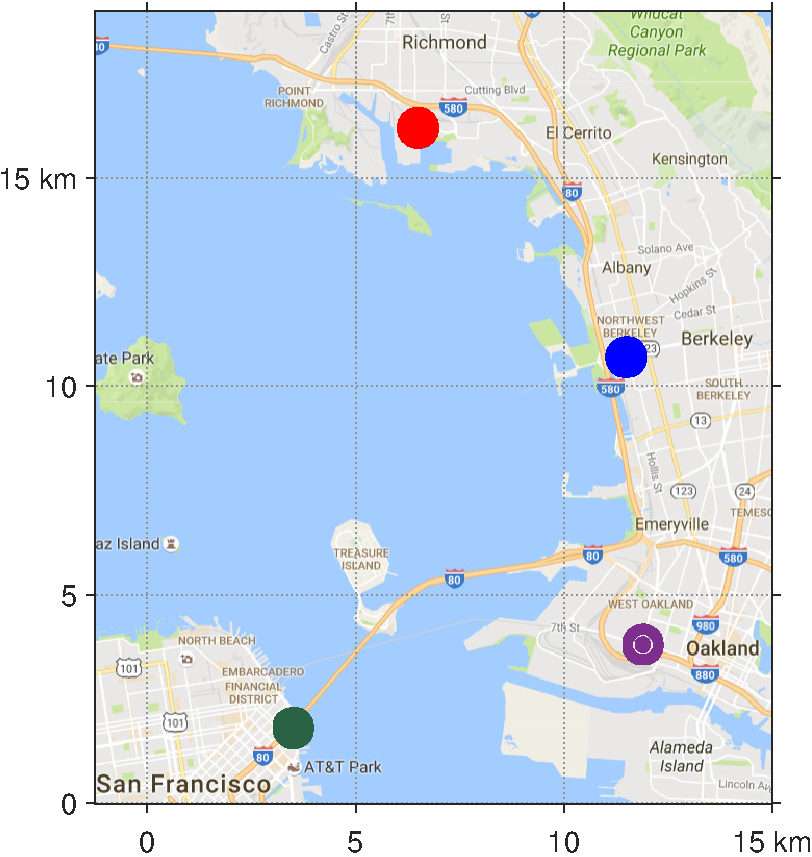
\includegraphics[width=\columnwidth]{figs/bayArea_setup}
  \caption{Multi-city simulation setup. A $300 km^2$ area of San Francisco Bay Area is used as the state-space for vehicles. STP vehicles fly to and from the four cities indicated by the four circles. The simulations are performed under the strong winds condition with $d_{r} = 11 m/s$.}
  \label{fig:bayArea_setup}
\end{figure}

Each box in Figure \ref{fig:bayArea_setup} represents a $25$ km$^2$ area. The vehicles are flying to and from the four cities indicated by the four circles. The origin and the destination of each vehicle is chosen randomly from these four cities. The vehicle dynamics are given by \eqref{eq:dyn_i}. We choose velocity and turn-rate bounds as $\underline{v} = 0$ m/s, $\bar{v} = 25$ m/s, $\bar\omega = 2$ rad/s. The disturbance bound is chosen as $d_{r} = 11$ m/s, which corresponds to \textit{strong breeze} on Beaufort wind force scale \cite{Windscale}. The scheduled time of arrival $\sta$ for vehicles are chosen as $5(i-1)$ s.

The goal of the vehicles is to reach their destinations while avoiding a collision with the other vehicles. The joint state space of this 200-vehicle system is 600-dimensional, making the joint trajectory planning and collision avoidance problem intractable for direct analysis. Therefore, we assign a priority order to vehicles and solve the trajectory planning problem sequentially.
% !TEX root = ../SPP_IoTjournal.tex
\subsection{Results \label{sec:bayArea_simResults}}
The trajectory planning for the vehicles is done using RTT algorithm, similar to that in Section \ref{sec:city_simResults}. The resulting trajectories of vehicles are shown in Figure \ref{fig:bayArea_d11sep5}. Once again, the vehicles remain clear of all other vehicles and reach their respective destinations. Given the relative separation between the scheduled times of arrival, the trajectories are predominately \textit{time-separated}, with roughly two lanes for each pair of cities (one for going from city A to city B and another for from city B to city A). A high-density of vehicles is achieved in the center since the 4 paths are intersecting in the center (Richmond-Oakland, Oakland-Richmond, Berkeley-San Francisco, San Francisco-Berkeley), but the SPP algorithm ensures safety despite this high-density, as shown in the zoomed-in version of center at an intermediate time when a large number of vehicles are passing through the central region (Figure \ref{fig:bayArea_d11sep5_zoomed}).  
%
\begin{figure*}[!htb]
 \centering
\begin{subfigure}{\columnwidth}
  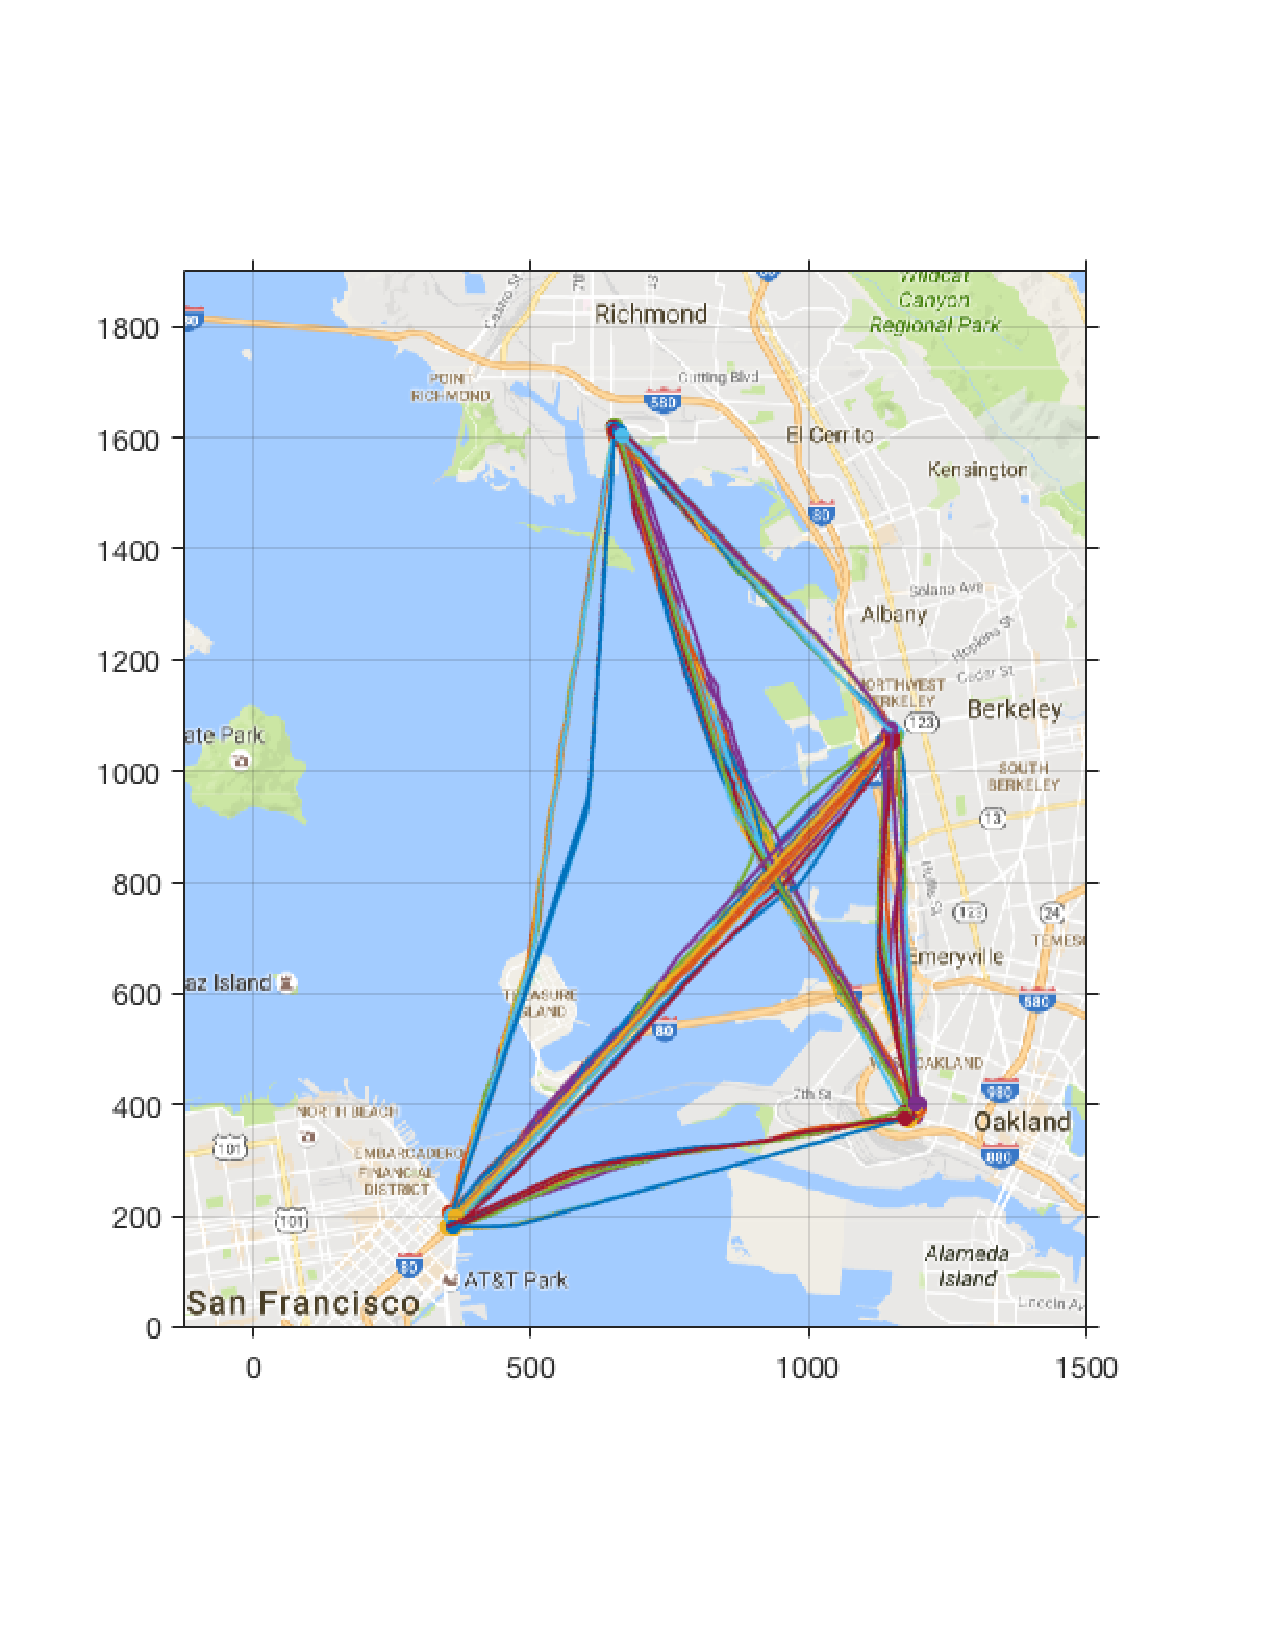
\includegraphics[width=\columnwidth]{figs/bayArea_d11sep5}
  \subcaption{}
  \label{fig:bayArea_d11sep5}
\end{subfigure}%
\begin{subfigure}{\columnwidth}
  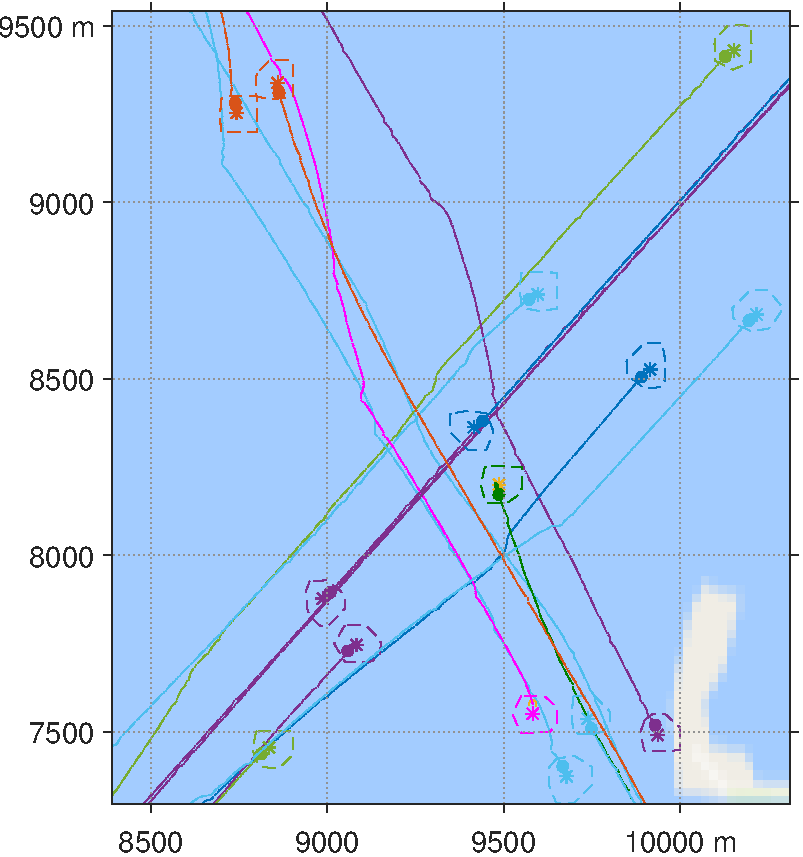
\includegraphics[width=\columnwidth]{figs/bayArea_d11sep5_zoomed}
  \subcaption{}
  \label{fig:bayArea_d11sep5_zoomed}
\end{subfigure}%
  \caption{(a) Trajectories obtained from the SPP algorithm for the multi-city simulation with $d_r = 11m/s$, $\sta_i = 5(i-1)$. (b) Zoomed-in version of the central area. A high density of vehicles is achieved at the center because of the intersection of several trajectories; however, the SPP algorithm still ensures that vehicles do not enter each other's danger zones and reach their destinations.} 
  \label{fig:bayArea_d11sep5_all}
\end{figure*}

Finally, we simulate the system for the case where $\sta_i = 0 ~\forall i$. As evident from Figure \ref{fig:bayArea_d11sep0}, we get multiple lanes between each pair of cities in this case and trajectories become predominately state-separated, as we expect based on the discussion in Section \ref{sec:city_distbEffect}.
\begin{figure}[t]
  \centering
  \includegraphics[width=\columnwidth]{"figs/bayArea_d11sep0"}
  \caption{Vehicle trajectories for $d_r = 11m/s$, $\sta_i = 0$. Since different vehicles have same scheduled times of arrival, a multiple-lane behavior is observed between every pair of cities.} 
  \label{fig:bayArea_d11sep0}
\end{figure}

The average trajectory computation time per vehicle is \SBnote{$XYZ$s} per vehicle on a \SBnote{$Blah Blah$} computing machine. Once again all the computation is done offline and only a lookup table query is required in real-time, which can be performed very efficiently. This simulation illustrates the scalability and the potential of deploying the SPP algorithm for provably safe path planning for large multi-vehicle systems.
% !TEX root = ../SPP_IoTjournal.tex
\subsection{Effect of Disturbance and Scheduled Time of Arrival \label{sec:city_distbEffect}}
In this section, we illustrate how the disturbance bound $d_r$ in \eqref{eq:dyn_i} and the realtive $\sta$s of vehicles affect the vehicle trajectories. For this purpose, we simulate the SPP algorithm for four additional scenarios:
\begin{itemize}
\item Case-0: $d_r = 6m/s$, $\sta_i = 0 ~\forall i$
\item Case-1: $d_r = 11m/s$, $\sta_i = 0 ~\forall i$
\item Case-2: $d_r = 6m/s$, $\sta_i = 5(i-1) ~\forall i$
\item Case-3: $d_r = 11m/s$, $\sta_i = 5(i-1) ~\forall i$
\item Case-4: $d_r = 11m/s$, $\sta_i = 10(i-1) ~\forall i$
\end{itemize}
The interpretation $\sta_i = 5(i-1)$ is that the scheduled time of arrival of any two consecutive vehicles is separated by 5s. $d_r = 6m/s$ and $d_r = 11m/s$ correspond to the moderate winds and strong winds respectively on Beaufort wind force scale \cite{Windscale}. 

Intuitively, as $d_r$ increases, it is harder for a vehicle to closely track a particular nominal trajectory, which results in a higher tracking error bound. \SBnote{Add the exact error bounds here.} Thus, the vehicles need to be separated more from each other in space to ensure that they do not enter each other's danger zones. This is also evident from comparing the results corresponding to Case-0 (Fig. \ref{fig:sf_d6sep0}) and Case-1 (Fig. \ref{fig:sf_d11sep0}). As the disturbance magnitude increases from $d_r = 6m/s$ (moderate winds) to $d_r = 11m/s$ (strong winds), the vehicles' trajectories get farther apart from each other. Since $\sta$ is same for all vehicles, the vehicles’ trajectories are still predominately \textit{state-separated} trajectories.

We next compare Case-0 and Case-2. The difference between these two cases is that vehicles have different $\sta$s in Case-2. When vehicles $\veh_i$ and $\veh_{j}$ ($j>i$) have same scheduled time of arrival and are going to the same destination, they are constrained to travel at the same time to make sure they reach the destination by the designtaed $\sta$. However, since $\veh_i$ is high-priority, it gets access to the optimal trajectory (in terms of the total time of tarvel to destination) and $\veh_{j}$ has to settle for a relatively sub-optimal trajectory. Thus, all vehicles going to a particular destination take different trajectories creating a ``band" of trajectories between the origin and the destination, as shown in Figure \ref{fig:sf_d6sep0}; the high-priority vehicles take a relatively straight path between the origin and the destination whereas the low-priority vehicles take a (relatively sub-optimal) curved path. If we think of an air highway between the origin and the destination, then vehicles take different lanes of that highway to reach the destination in Case-0. Thus, the trajectories of vehicles in this case are \textit{state-separated}. However, when $\sta_j > \sta_i$, then $\veh_j$ is not bound to travel at the same time as $\veh_i$; it can wait for $\veh_i$ to depart and take a shorter path later on. Thus, vehicles travel in a single (optimal) lane in this case, as shown in Figure \ref{fig:sf_d6sep5}. In other words, they take the same trajectory to the destination, but at different times. Thus, the trajectories of vehicles in this case are \textit{time-separated}. 

Note that the exact number of lanes depends on both the disturbance and relative $\sta$s. As disturbance increases, the vehicles need to be separated more from each other to ensure safety. The relative difference in $\sta$s should be able to ensure this separation if they were to take the same lane. As shown in Figure \ref{fig:sf_d11sep5}, a difference of 5s in $\sta$s is not sufficient to achieve a single lane behavior for strong winds. However, the number of lanes are significantly less than that in Case-1 (Fig. \ref{fig:sf_d11sep0}). Finally, a difference of 10s in $\sta$s ensure that we get the single lane behavior even in the presence of strong winds, leading to \textit{time-separated} trajectories. \SBnote{Add link to the simulation videos for each result.}

Overall, the relative magnitude of disturbance and scheduled times of arrival separation determines the number of lanes and type of trajectories that emerge out of the SPP algorithm. For a fixed disturbance magnitude, as the relative separation in the scheduled times of arrival of vehicles increases, the number of lanes between a pair of origin and destination decreases, and more and more tarjectories become time-separated. On the other hand, for a fixed relative separation in the scheduled times of arrival of vehicles, as the disturbnace magnitude increases, the number of lanes between a pair of origin and destination increases, and more and more tarjectories become state-separated.
%
\begin{figure*}[!htb]
 \centering
\begin{subfigure}{\columnwidth}
  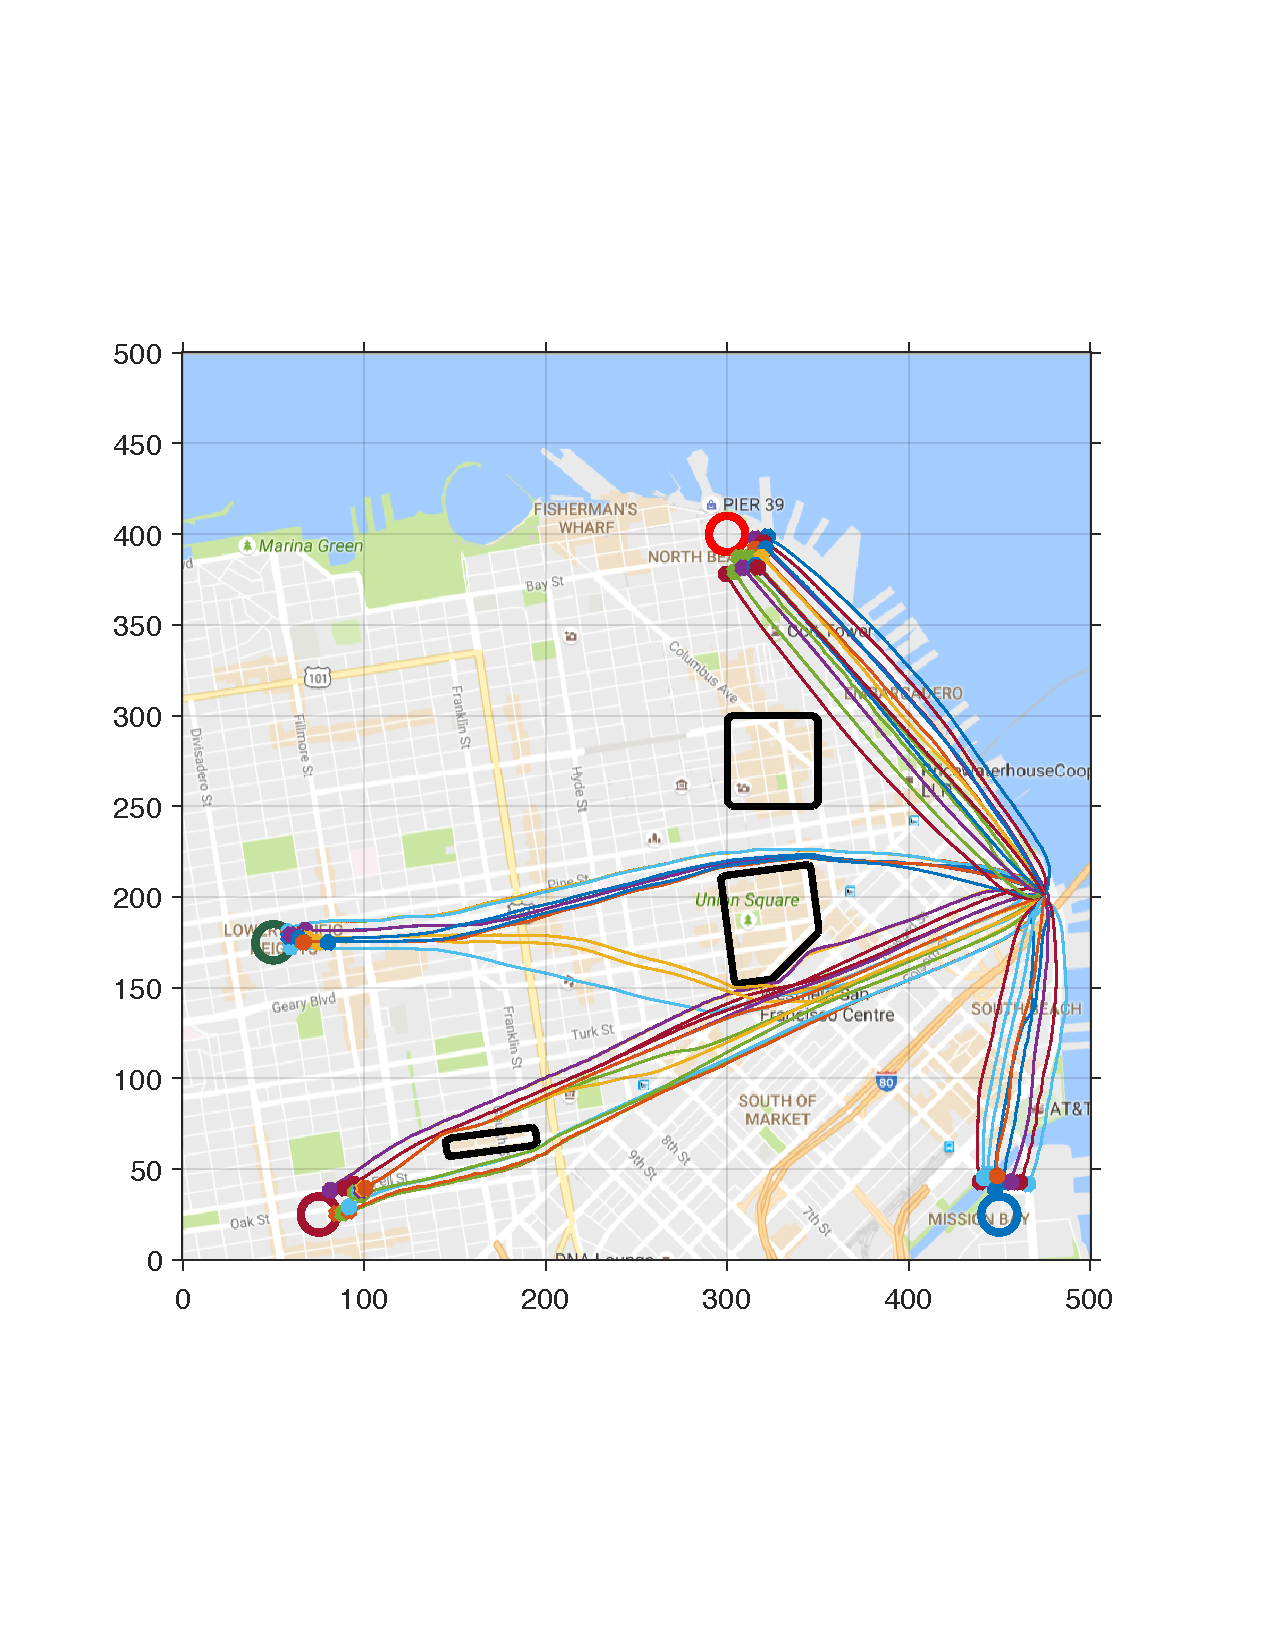
\includegraphics[width=\columnwidth]{figs/sf_d6sep0}
  \subcaption{Case-0: $d_r = 6m/s$, $\sta_i = 0$}
  \label{fig:sf_d6sep0}
\end{subfigure}%
\begin{subfigure}{\columnwidth}
  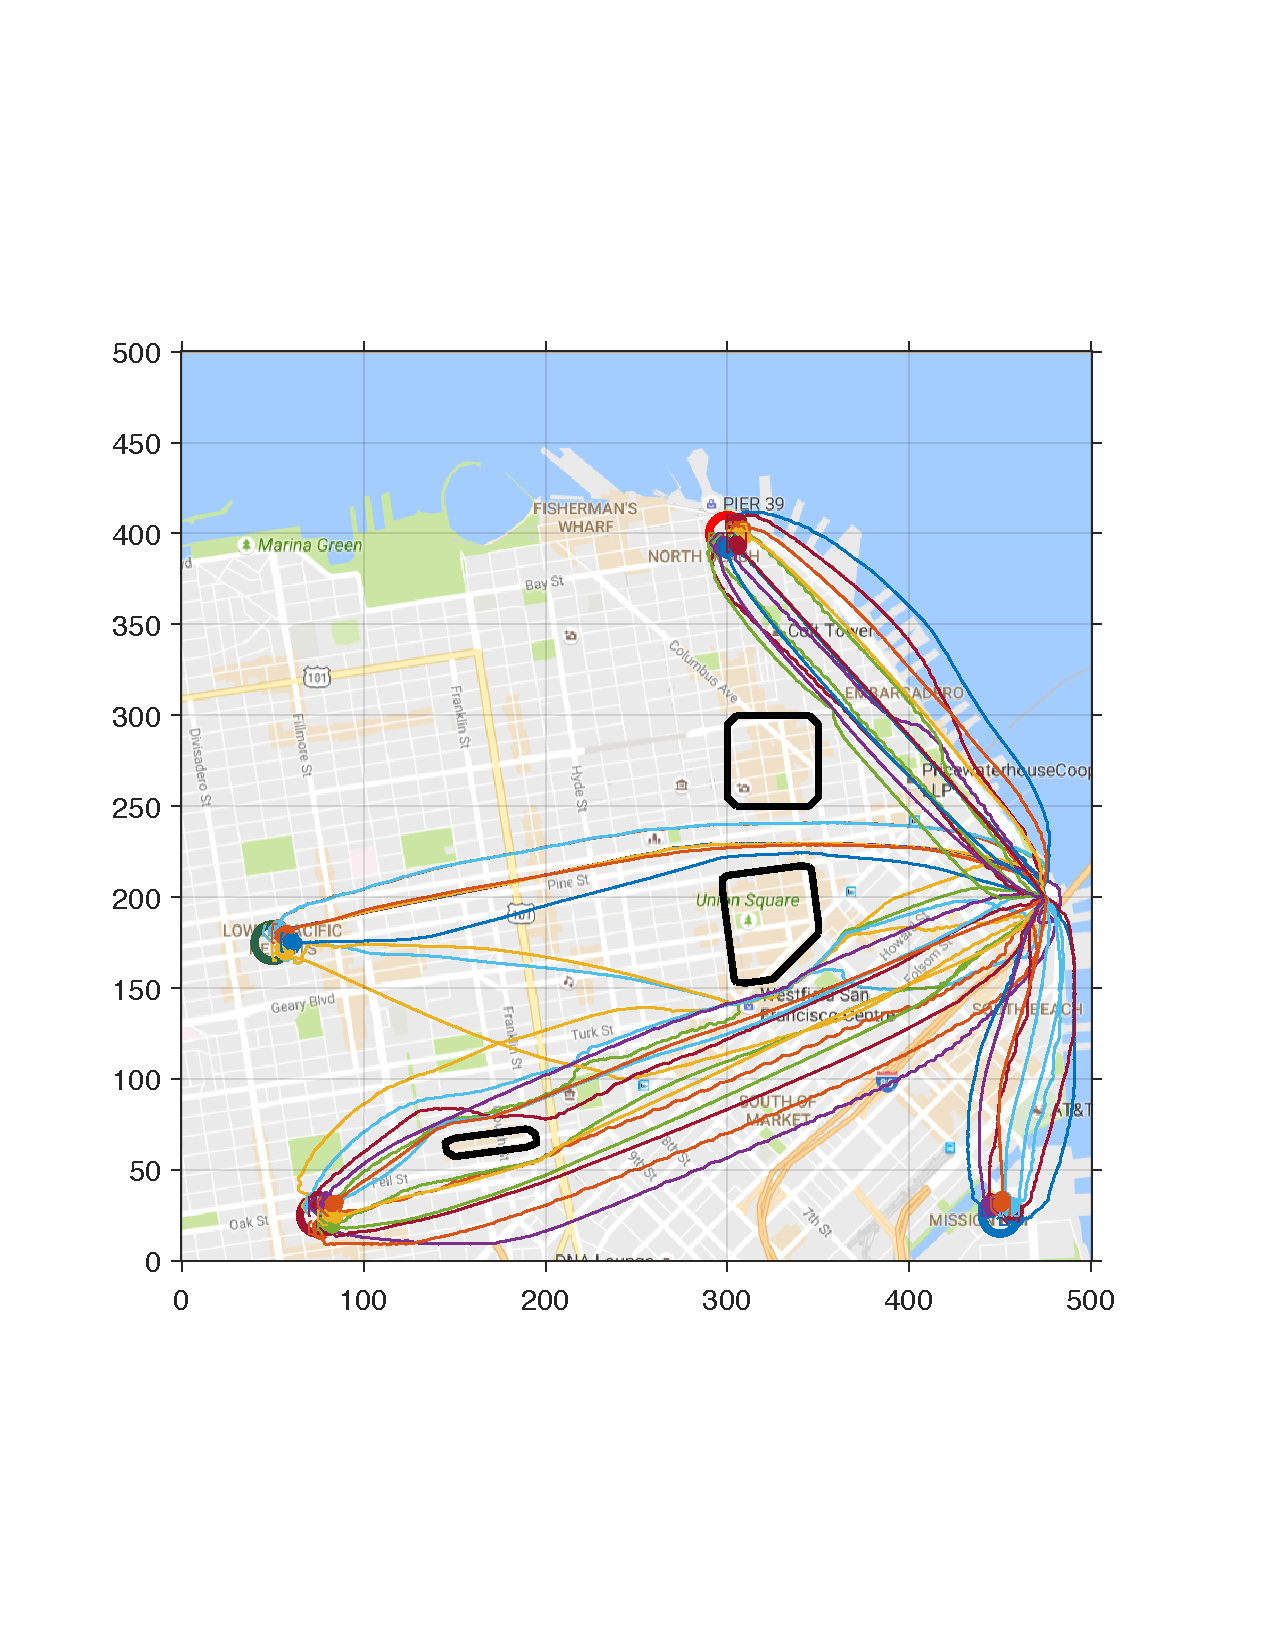
\includegraphics[width=\columnwidth]{figs/sf_d11sep0}
  \subcaption{Case-1: $d_r = 11m/s$, $\sta_i = 0$}
  \label{fig:sf_d11sep0}
\end{subfigure}%

\begin{subfigure}{\columnwidth}
  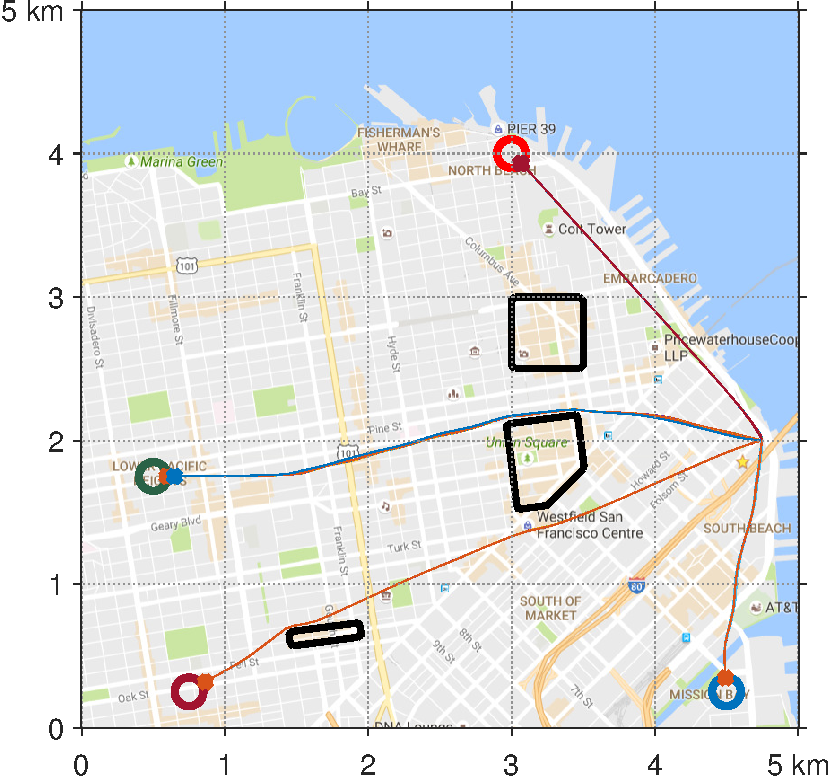
\includegraphics[width=\columnwidth]{figs/sf_d6sep5}
  \subcaption{Case-2: $d_r = 6m/s$, $\sta_i = 5(i-1)$}
  \label{fig:sf_d6sep5}
\end{subfigure}%
\begin{subfigure}{\columnwidth}
  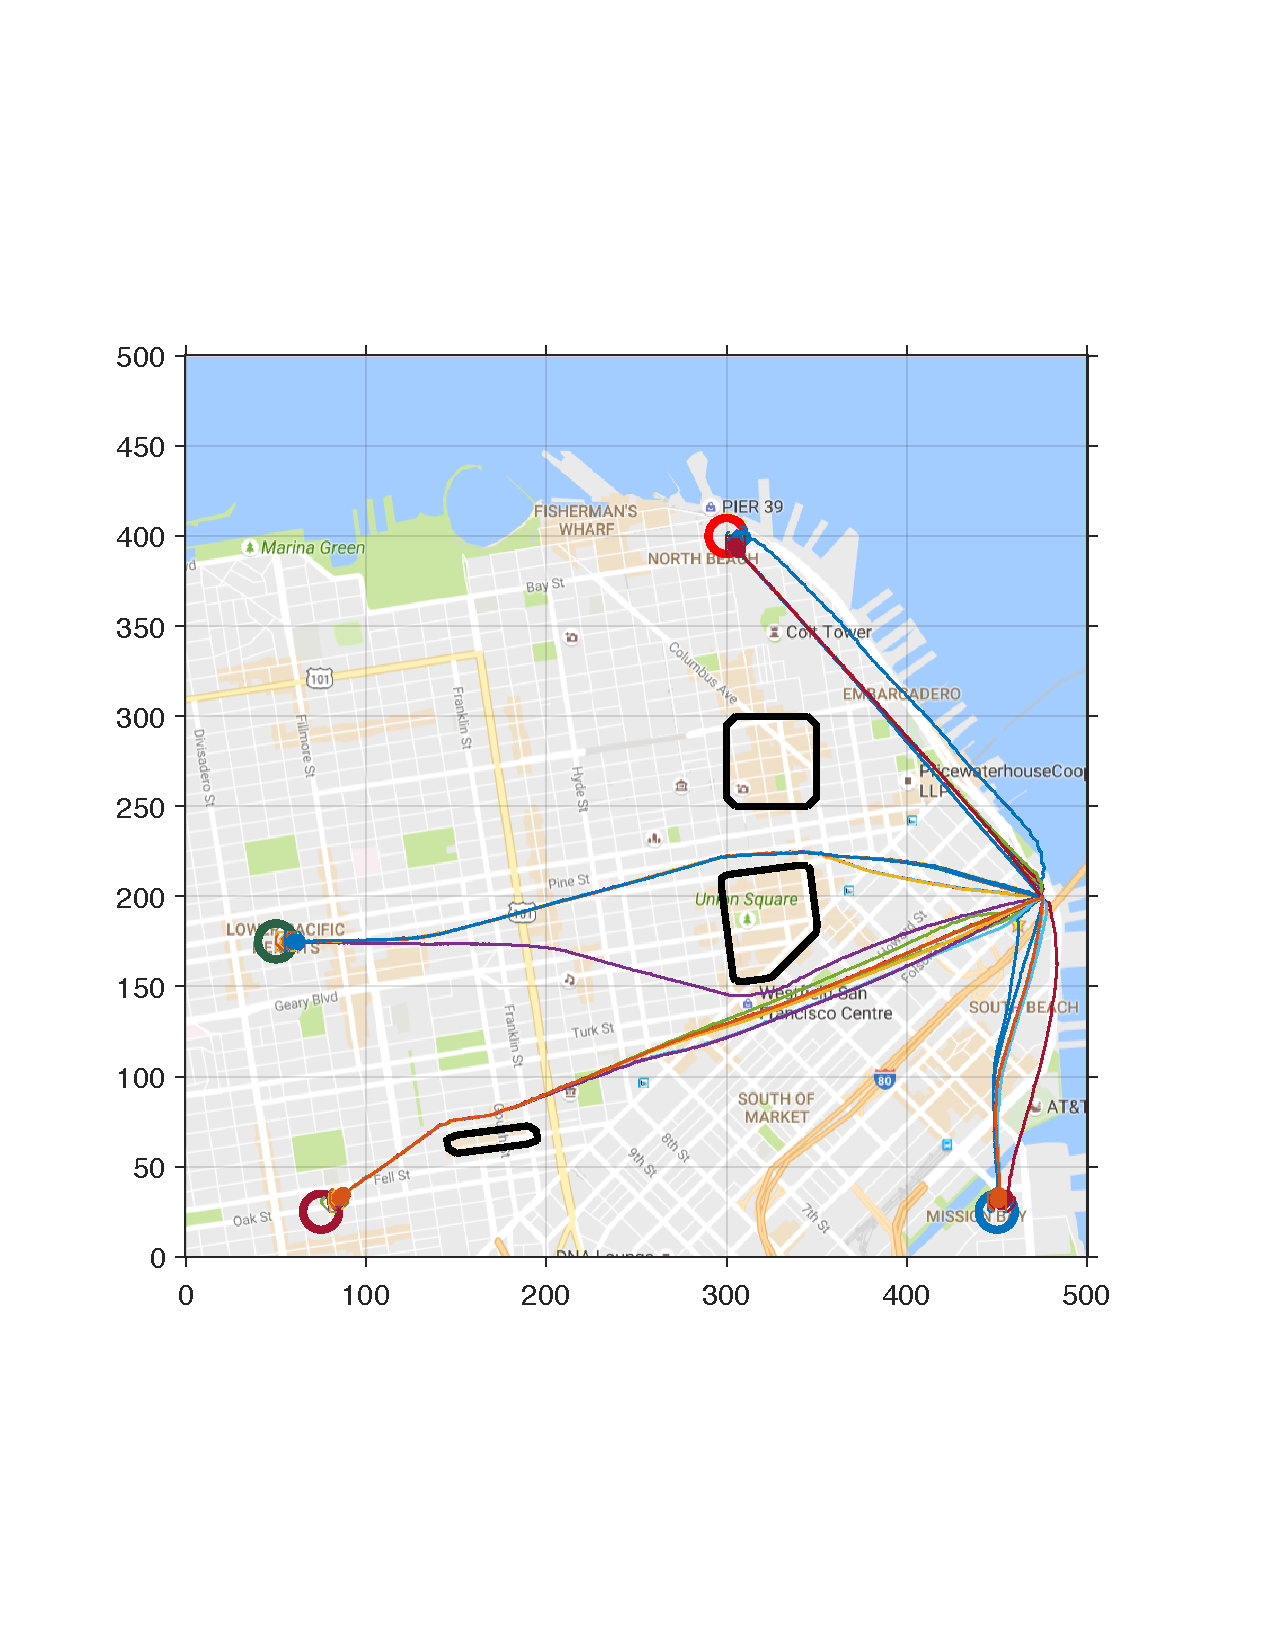
\includegraphics[width=\columnwidth]{figs/sf_d11sep5}
  \subcaption{Case-3: $d_r = 11m/s$, $\sta_i = 5(i-1)$}
  \label{fig:sf_d11sep5}
\end{subfigure}%
\caption{Effect of the disturbance magnitude and the scheduled times of arrival on vehicle trajectories. All trajectories are simulated under uniformly random disturbance. The relative separation in the scheduled times of arrival of vehicles determines the number of lanes between a pair of origin and destination, and more and more tarjectories become time-separated as this relative separation increases. The disturbnace magnitude determines the relative separation between different lanes, and more and more tarjectories become state-separated as the disturbance increases. }
\label{fig:trajectories_sf}
\end{figure*}

\begin{figure}[t]
  \centering
  \includegraphics[width=\columnwidth]{"figs/sf_d11sep10"}
  \caption{Vehicle trajectories for Case-4: $d_r = 11m/s$, $\sta_i = 10(i-1)$. Since different vehicles have different scheduled times of arrival, there is a single lane between every origin-destination pair.} 
  \label{fig:sf_d11sep10}
\end{figure}

% Bay Area level Simulations
% !TEX root = ./SPP_IoTjournal.tex
\section{Simulations \label{sec:simulations}}
We now illustrate the proposed algorithm using a fifty-vehicle example. 

\subsection{Setup \label{sec:simSetup}}
Our goal is to simulate a scenario where UAVs are flying through an urban environment. This setup can be representative of many UAV applications, such as package delivery, aerial surveillance, etc. For this purpose, we grid San Francisco (SF) city in California, US and use it as our state space, as shown in Figure \ref{fig:sf_setup}. 
\begin{figure}[H]
  \centering
  \includegraphics[width=\columnwidth]{"figs/sf_setup"}
  \caption{Simulation setup. A $25 km^2$ area of San Francisco city is used as the state-space for vehicles. SPP vehicles originate from the Blue star and go to one of the four destinations, denoted by circles. Tall buildings in the downtown area are used as static obstacles, represented by the black contours.}
  \label{fig:sf_setup}
\end{figure}
Each box in Figure \ref{fig:sf_setup} represents a $500m \times 500m$ area of SF. The origin point for the vehicles is denoted by the Blue star. Four different areas in the city are chosen as the destinations for the vehicles. Mathematically, the target sets $\targetset_i$ of the vehicles are circles of radius $r$ in the position space, i.e. each vehicle is trying to reach some desired set of positions. In terms of the state space $\state_i$, the target sets are defined as
\begin{equation}
\label{eq:target_sim}
\targetset_i = \{\state_i: \|\pos_i - c_i\|_2 \le r\}
\end{equation}
\noindent where $c_i$ are centers of the target circles. In this simulation, we use $r = 100m$. The four targets are represented by four circles in Figure \ref{fig:sf_setup}. The destination of each vehicle is chosen randomly from these four destinations. Finally, tall buildings in downtown San Francisco are used as static obstacles for the SPP vehicles, denoted by black contours in Figure \ref{fig:sf_setup}.

For this simulation, we use the following dynamics for each vehicle:
\begin{equation}
\label{eq:dyn_i}
\begin{aligned}
\dot{\pos}_{x,i} &= v_i \cos \theta_i + d_{x,i} \\
\dot{\pos}_{y,i} &= v_i \sin \theta_i + d_{y,i}\\
\dot{\theta}_i &= \omega_i, \\
\underline{v} \le v_i \le \bar{v}, & ~|\omega_i| \le \bar{\omega}, ~\|(d_{x,i}, d_{y,i}) \|_2 \le d_{r},
\end{aligned}
\end{equation}
\noindent where $\state_i = (\pos_{x,i}, \pos_{y,i}, \theta_i)$ is the state of vehicle $\veh_i$, $\pos_i = (\pos_{x,i}, \pos_{y,i})$ is the position, $\theta_i$ is the heading, and $d = (d_{x,i}, d_{y,i})$ represents $\veh_i$'s disturbances, for example wind, that affect its position evolution. The control of $\veh_i$ is $u_i = (v_i, \omega_i)$, where $v_i$ is the speed of $\veh_i$ and $\omega_i$ is the turn rate; both controls have a lower and upper bound. To make our simulations as close as possible to real scenarios, we choose velocity and turn-rate bounds as $\underline{v} = 0m/s, \bar{v} = 25m/s, \bar\omega = 2 rad/s$, aligned with the modern UAV specs \cite{UAVspecs1, UAVspecs2}. The disturbance bound is chosen as $d_{r} = 6 m/s$, which corresponds to \textit{moderate winds} on Beaufort wind force scale \cite{Windscale}. Note that we have used same dynamics and input bounds across all vehicles for clarity of illustration; however, our method can easily handle more general systems of the form in which the vehicles have different control bounds and dynamics.

The goal of the vehicles is to reach their destinations while avoiding a collision with the other vehicles or the static obstacles. The vehicles also need to account for the possibility of the presence of an intruder for a maximum duration of $\iat = 10s$, whose dynamics are given by \eqref{eq:dyn_i}. The joint state space of this fifty-vehicle system is 150-dimensional (150D), making the joint path planning and collision avoidance problem intractable for direct analysis using HJ reachability. Therefore, we assign a priority order to vehicles and solve the path planning problem sequentially. For this simulation, we assign a random priority order to fifty vehicles and use the algorithm proposed in Section \ref{sec:intruder} to compute a separation between SPP vehicles so that they do not collide with each other or the intruder. 

\subsection{Results \label{sec:simResults}}
In this section, we present the simulation results for $\nva = 3$; occassionally, we also compare the results for different $\nva$s to highlight some key points about the proposed algorithm. As per Algorithm \ref{alg:intruder}, we begin with computing the avoid region $\brs^{\text{A}}_{i}(0, \iat)$. To compute the avoid region, relative dynamics between $\veh_i$ and $\veh_{\intr}$ are required. Given dynamics in \eqref{eq:dyn_i}, the relative dynamics are given by \cite{Mitchell05}:
\begin{equation}
\label{eq:reldyn_i}
\begin{aligned}
\dot{\pos}_{x, \intr, i} &= v_{\intr} \cos \theta_{\intr, i} - v_i + \omega_i {\pos}_{y, \intr, i} + d_{x,i} + d_{x,\intr}\\
\dot{\pos}_{y, \intr, i} &= v_i \sin \theta_{\intr, i} - \omega_i {\pos}_{x, \intr, i} + d_{y,i} + d_{y,\intr}\\
\dot{\theta}_{\intr, i} &= \omega_{\intr} - \omega_i,
\end{aligned}
\end{equation}    
where $\state_{\intr, i} = (\pos_{x, \intr, i}, \pos_{y, \intr, i}, \theta_{\intr, i})$ is the relative state between $\veh_{\intr}$ and $\veh_i$. Given relative dynamics, the avoid region can be computed using \eqref{eqn:avoidBRS}. For all the BRS and FRS computations in this simulation, we use Level Set Toolbox \cite{Mitchell07b}. Also, since the vehicle dynamics' are same across all vehicles, we will omit the vehicle index from sets wherever applicable. The avoid region $\brs^{\text{A}}(0, \iat)$ for SPP vehicles is shown in Figure \ref{fig:MaxMin}.
\begin{figure}[H]
  \centering
  \includegraphics[width=\columnwidth]{"figs/bufferRegion_steps"}
  \caption{Base obstacle $\boset(t)$ , Avoid region $\brs^{\text{A}}(0, \iat)$, Separation region $\sep(t)$ and Relative buffer region $\brs^{\text{B}}(0, \brd)$ for vehicles. The three axes represent three states of the vehicles.}
  \label{fig:MaxMin}
\end{figure}
As long as $\veh_{\intr}$ starts outside the avoid region, $\veh_i$ is guarnateed to avoid the intruder for a duration of $\iat$. Given $\brs^{\text{A}}(0, \iat)$, we can compute the minimum required detection range $\dsen$ given by \eqref{eqn:sen_distance}, which turns out to be 100m in this case. So as long as the vehicles can detect the intruder within 100m, the proposed algorithm guarantees collision avoidance with the intruder as well as a safe transit to their respective destinations.   

Next, we compute the separation and buffer regions between vehicles. For the computation of base obstacles, we use RTT method \cite{Bansal2017}. In RTT method, a nominal trajectory is declared by the higher priority vehicles, which is then guaranteed to be tracked with some known error bound in the presence of disturbances. The base obstacles are thus given by a ``bubble" around the nominal trajectory. For further details of RTT method, we refer the interested readers to Section 4C in \cite{Bansal2017}. The position tracking error bound obtained for the strong wind conditions is $5$m. The overall base obstacle $\boset$ around the nominal tarjectory point $(0, 0, 0)$ is shown in Figure \ref{fig:MaxMin}. Thus, the base obstacles induced by a higher priority vehicle are given by this set augmented on the nominal trajectory, the trajectory that a vehicle will follow if the intruder never appears in the system, and is obtained by executing the control policy ${\ctrl^{\text{PP}}_{i}}(\cdot)$ in \eqref{eqn:PPPolicy}.

Given $\boset$ and $\brs^{\text{A}}(0, \iat)$, we compute the separation region $\sep$ as defined in \eqref{eqn:sepRegion_case1}. Relative buffer region $\brs^{\text{B}}(0, \brd)$, defined in \eqref{eqn:buffBRS_case1}, is computed next. The results are shown in Figure \ref{fig:MaxMin}. Note that since $\nva = 3$, $\brd = 10/3$. Finally, we compute the buffer region as defined in \eqref{eqn:buffRegion_case1}. The resultant buffer region is shown in Blue in Figure \ref{fig:buffRegions}. Thus, if $\veh_j$ is inside the base obstacle set shown in Figure \ref{fig:MaxMin} and $\veh_i$ is outside the Blue region in Figure \ref{fig:buffRegions}, we can ensure that the intruder will have to spend a duration of atleast $\brd$ to go from the boundary of the avoid region of $\veh_j$ to the boundary of the avoid region of $\veh_i$. 
\begin{figure}[H]
  \centering
  \includegraphics[width=\columnwidth]{"figs/bufferRegions_3D"}
  \caption{Buffer regions for different $\nva$ (best visualized with colors). As $\nva$ decreases, a larger buffer is required between vehicles to ensure that the intruder spends more time while traveling through this buffer region so that it forces fewer vehicles to apply an avoidnace maneuver.}
  \label{fig:buffRegions}
\end{figure}
We also computed the buffer regions for $\nva = 2$ and $\nva = 4$. The results are shown in Figure \ref{fig:buffRegions}. Top-down views of these 3D sets are shown in Figure \ref{fig:buffRegions_td}. As evident from the figures, a bigger buffer region is required between vehicles when $\nva$ is smaller. Intuitively, when $\nva$ is smaller, a larger buffer is required to ensure that the intruder spends more time ``traveling" through this buffer region so that it can affect fewer vehicles.             
\begin{figure}[H]
  \centering
  \includegraphics[width=\columnwidth]{"figs/bufferRegions_topdown"}
  \caption{Top-down view of the buffer regions for different $\nva$ shown in Figure {fig:buffRegions} (best visualized with colors). As $\nva$ decreases, $\brd$ increase and a larger buffer is required between vehicles.}
  \label{fig:buffRegions_td}
\end{figure}

Similarly, we sequentially computed the obstacles induced by the higher priority vehicles for each vehicle, i.e. $\obsset(\cdot)$, and the corresponding nominal trajectories, obtained by executing the control policy $\ctrl^{\text{PP}}(\cdot)$ defined in \eqref{eqn:PPPolicy}. The nominal trajectory thus corresponds to the trajectory that a vehicle will follow if the intruder does not appear in the system. The nominal trajectories and the overall obstacles for different vehicles at any arbitrary time are shown in Figure \ref{fig:trajObsSim} for the case $\nva = 3$. \SBnote{Report the min, max and average of space-time reservation and actual flight time of the vehicles here.} The nominal trajectories (solid lines) are well separated from each other to ensure safe transition even during a worst-case intruder ``attack". The dashed circle around a vehicle denote the overall obstacle induced by that vehicle for the lower priority vehicles. As expected, all vehicles are outside each other's induced obstacles, as well as static obstacles. %Accounting for this worst-case behavior makes our reachability analysis conservative and this limitation is discussed more Section \ref{sec:discuss}.
Note that in the absence of an intruder the vehicles transit successfully to their destinations with control policy $\ctrl^{\text{PP}}(\cdot)$, but they can deviate from the shown nominal trajectories if an intruder appears in the system.
\begin{figure}[H]
  \centering
  \includegraphics[width=\columnwidth]{"figs/nomTraj"}
  \caption{Nominal trajectories and induced obstacles by different vehicles. The nominal trajectories (solid lines) are well separated from each other to ensure safe transition even in the presnece of an intruder.}
  \label{fig:trajObsSim}
\end{figure}

Finally, in Figure \ref{fig:trajComparison}, we show that how the avoidance control can cause a deviation from the nominal trajectory. As evident from the figure, if vehicle doesn't apply the avoidnace maneuver and continue to track the nominal trajectory in the presence of an intruder, this might lead to a collision with the intruder. On the other hand, if the vehicle applies the avoidance policy $\ctrl^{\text{A}}(\cdot)$, it can successfully avoid a collision with the intruder. \SBnote{Add the figure here.} 

Under the proposed algorithm, the intruder will affect maximum number of vehicles ($\nva$ vehicles), when it appears at the boundary of the avoid region of a vehicle, immediately ``travels" through the buffer region between vehicles and reach the boundary of the avoid region of another vehicle at $\tsa + \brd$ and then the boundary of the avoid region of another vehicle at $\tsa + 2\brd$ and so on. This strategy will make sure that the intruder affects $\nva$ vehicles during a duration of $\iat$. However, the relative buffer region between vehicles is computed under the assumption that both the SPP vehicle and the intruder are trying to collide with each other, which is not necessarily true as a vehicle will be applying the control policy $\ctrl^{\text{PP}}(\cdot)$ unless the intruder forces it to apply an avoidance maneuver, so it is very likely that the intruder will affect less than $\nva$ vehicles even with this best strategy to affect maximum vehicles. This is also evident from Figures \ref{fig:bestStrategy1} and \ref{fig:bestStrategy1}. 
\SBnote{To-dos:
\begin{itemize}
\item Add the explanation of what is happening in figures once we have the figures. Make time points and vehicle numbers precise
\item Explain which vehicles need to replan their trajectories once the intruder disappears in each case. Explicitly define the set. 
\item Mention the avoid start times of vehicles.
\end{itemize}
}  

In Case-1, the intruder forces all 3 vehicles to apply an avoidance maneuver so we need to replan the trajectories of $3 (= \nva)$ vehicles once the intruder disappears. However, a vehicle applies control policy $\ctrl^{\text{PP}}(\cdot)$ while the intruder is traveling through the buffer region, which may not necessarily correspond to the policy that the vehicle will use to \textit{deliberately} collide with the intruder, unlike assumed during the computation of the set $\brs^{\text{B}}(0, \brd)$. Thus, at $\tsa + \brd$, the intruder may not reach the boundary of the avoid region of $\veh_{XY}$.         

\subsection{Discussion \label{sec:discuss}}
The shown simulations illustrate the effectiveness of reachability in ensuring that the SPP vehicles safely reach their respective destinations even in the presence of an intruder. However, they also highlight some of the conservatism that is in-built in the reachability analysis due to the worst case analysis. For example, in the proposed algorithm, we assume the worst-case disturbances and intruder behavior while computing the buffer region and induced obstacles, which results in a large separation between vehicles and hence a lower vehicle density overall, as evident from Figure {fig:trajObsSim}. Similarly, while computing the relative buffer region, we assumed that a vehicle is \textit{deliberatley} trying to collide with the intruder so we once again consider the worst case scenario, as the vehicle will only be applying the nominal control strategy $\ctrl^{\text{PP}}(\cdot)$, which may not be same as the worst-case control strategy. Therefore, even though this worst-case analysis is essential to guarantee safety regardless the actions of SPP vehicles, the intruder and disturbances, a probabilistic safety analysis, that can overocme some of this conservatism, might be more suitable in practical applications.
% !TEX root = ../../STP_IoTjournal.tex
\subsection{Setup \label{sec:bayArea_simSetup}}
We grid the San Francisco Bay Area in California, US and use it as our state space, as shown in Figure \ref{fig:bayArea_setup}. We consider the UAVs flying to and from four cities: Richmond, Berkeley, Oakland, and San Francisco. The blue region in Fig. \ref{fig:bayArea_setup} represents bay. This environment is different from the city environment in Section \ref{sec:city_sim} in that now the UAVs need to fly for longer distances and through a high-density vehicle environment with strong winds, but have very few static obstacles like tall buildings.    
%
\begin{figure}
  \centering
  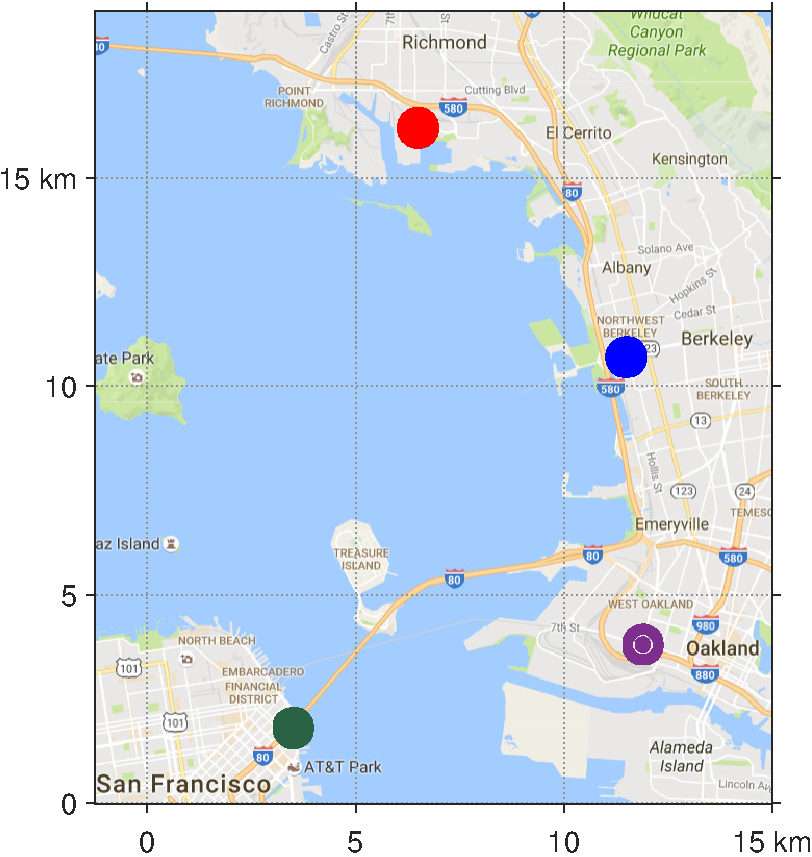
\includegraphics[width=\columnwidth]{figs/bayArea_setup}
  \caption{Multi-city simulation setup. A $300 km^2$ area of San Francisco Bay Area is used as the state-space for vehicles. STP vehicles fly to and from the four cities indicated by the four circles. The simulations are performed under the strong winds condition with $d_{r} = 11 m/s$.}
  \label{fig:bayArea_setup}
\end{figure}

Each box in Figure \ref{fig:bayArea_setup} represents a $25$ km$^2$ area. The vehicles are flying to and from the four cities indicated by the four circles. The origin and the destination of each vehicle is chosen randomly from these four cities. The vehicle dynamics are given by \eqref{eq:dyn_i}. We choose velocity and turn-rate bounds as $\underline{v} = 0$ m/s, $\bar{v} = 25$ m/s, $\bar\omega = 2$ rad/s. The disturbance bound is chosen as $d_{r} = 11$ m/s, which corresponds to \textit{strong breeze} on Beaufort wind force scale \cite{Windscale}. The scheduled time of arrival $\sta$ for vehicles are chosen as $5(i-1)$ s.

The goal of the vehicles is to reach their destinations while avoiding a collision with the other vehicles. The joint state space of this 200-vehicle system is 600-dimensional, making the joint trajectory planning and collision avoidance problem intractable for direct analysis. Therefore, we assign a priority order to vehicles and solve the trajectory planning problem sequentially.
% !TEX root = ../SPP_IoTjournal.tex
\subsection{Results \label{sec:bayArea_simResults}}
The trajectory planning for the vehicles is done using RTT algorithm, similar to that in Section \ref{sec:city_simResults}. The resulting trajectories of vehicles are shown in Figure \ref{fig:bayArea_d11sep5}. Once again, the vehicles remain clear of all other vehicles and reach their respective destinations. Given the relative separation between the scheduled times of arrival, the trajectories are predominately \textit{time-separated}, with roughly two lanes for each pair of cities (one for going from city A to city B and another for from city B to city A). A high-density of vehicles is achieved in the center since the 4 paths are intersecting in the center (Richmond-Oakland, Oakland-Richmond, Berkeley-San Francisco, San Francisco-Berkeley), but the SPP algorithm ensures safety despite this high-density, as shown in the zoomed-in version of center at an intermediate time when a large number of vehicles are passing through the central region (Figure \ref{fig:bayArea_d11sep5_zoomed}).  
%
\begin{figure*}[!htb]
 \centering
\begin{subfigure}{\columnwidth}
  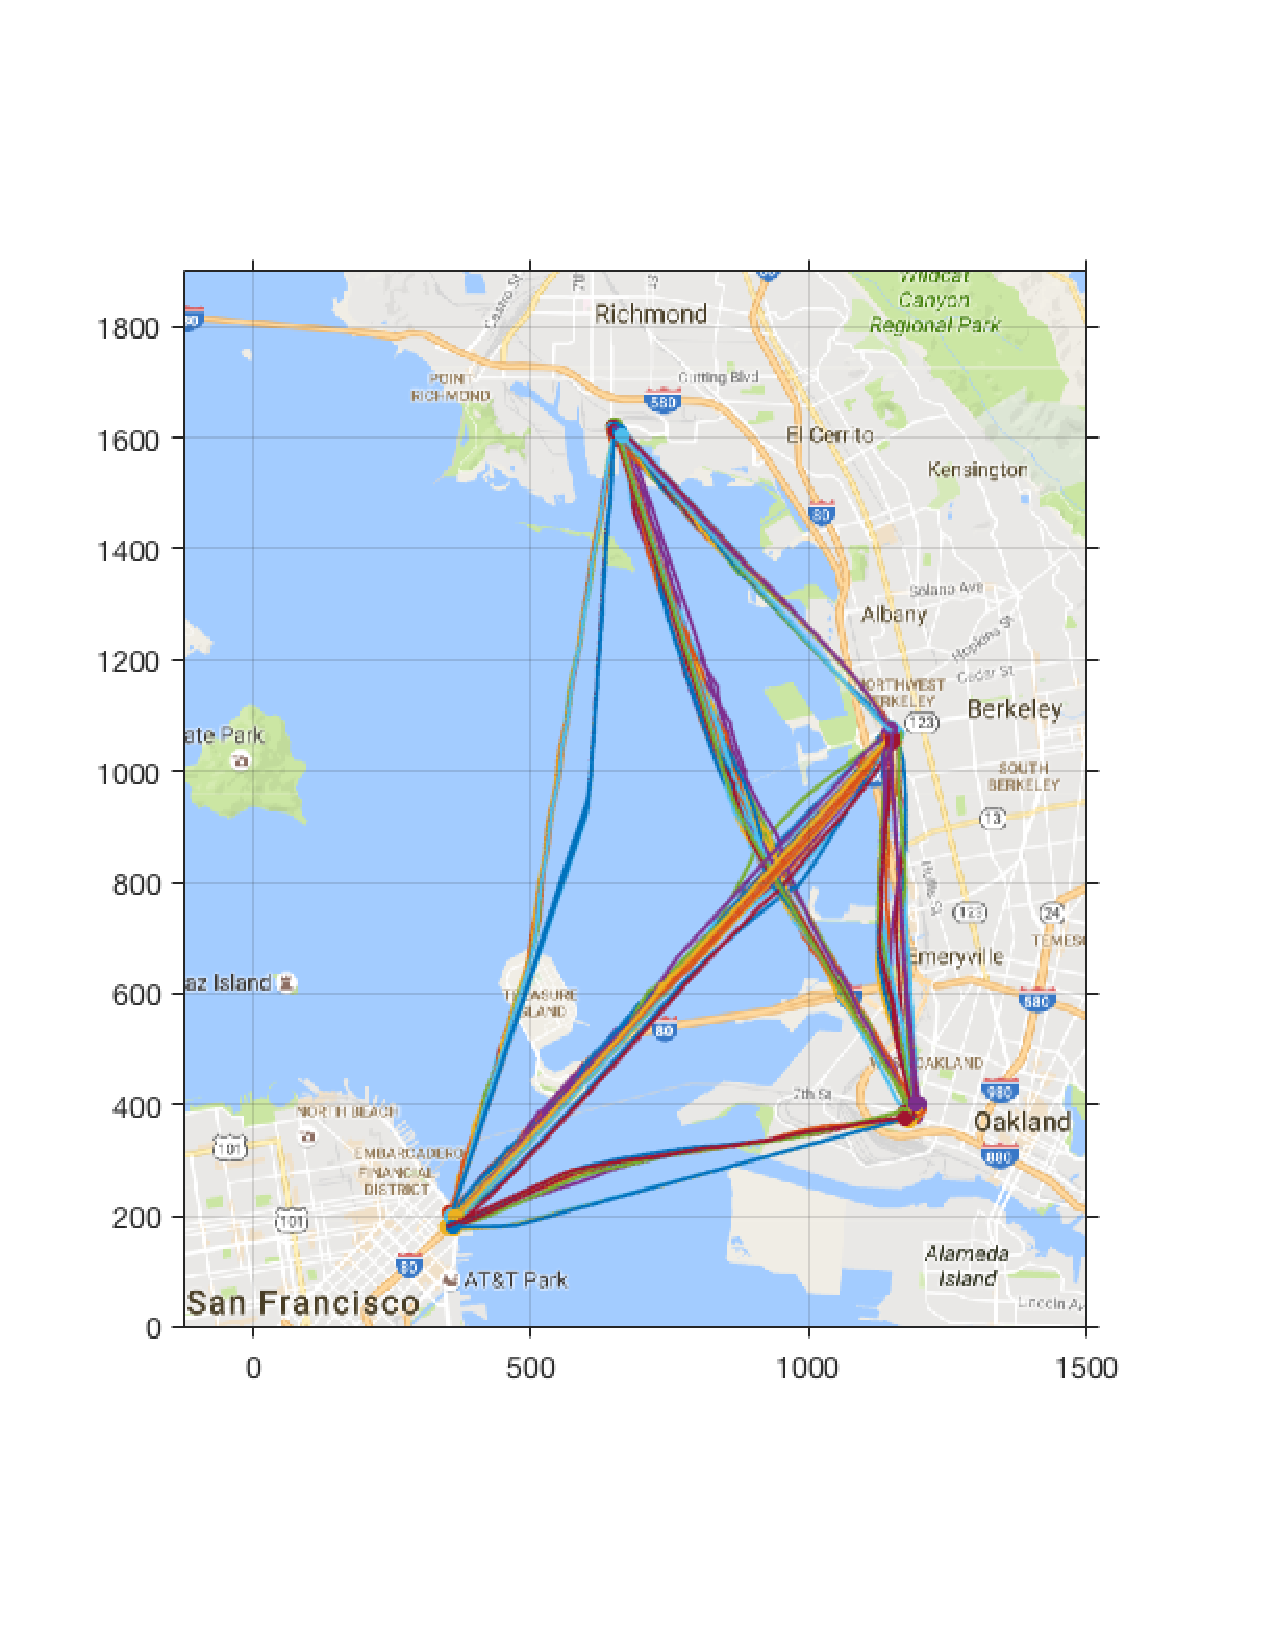
\includegraphics[width=\columnwidth]{figs/bayArea_d11sep5}
  \subcaption{}
  \label{fig:bayArea_d11sep5}
\end{subfigure}%
\begin{subfigure}{\columnwidth}
  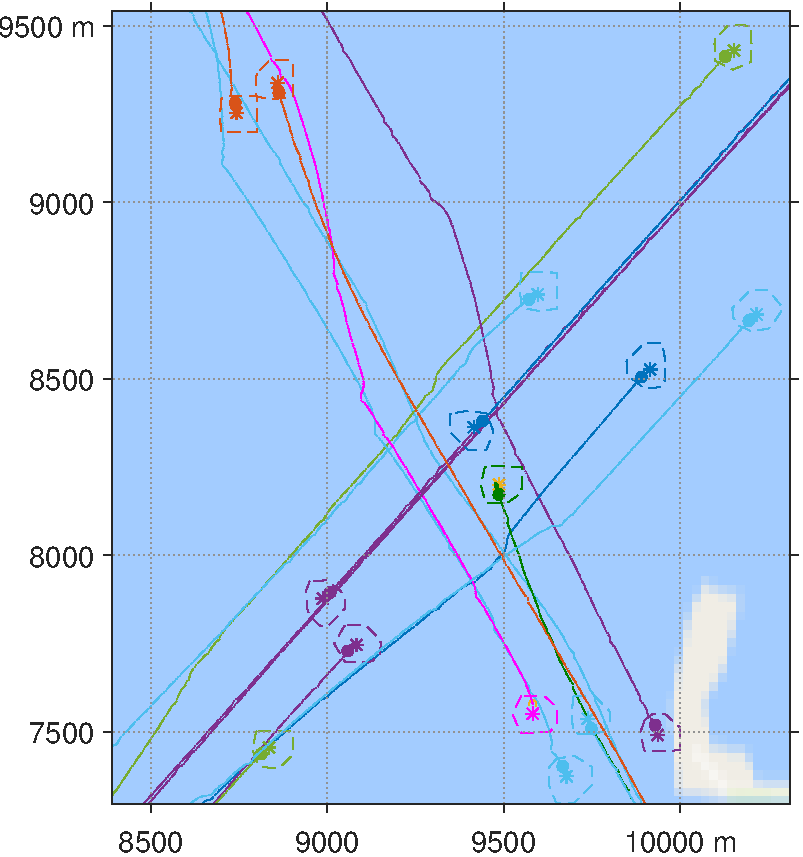
\includegraphics[width=\columnwidth]{figs/bayArea_d11sep5_zoomed}
  \subcaption{}
  \label{fig:bayArea_d11sep5_zoomed}
\end{subfigure}%
  \caption{(a) Trajectories obtained from the SPP algorithm for the multi-city simulation with $d_r = 11m/s$, $\sta_i = 5(i-1)$. (b) Zoomed-in version of the central area. A high density of vehicles is achieved at the center because of the intersection of several trajectories; however, the SPP algorithm still ensures that vehicles do not enter each other's danger zones and reach their destinations.} 
  \label{fig:bayArea_d11sep5_all}
\end{figure*}

Finally, we simulate the system for the case where $\sta_i = 0 ~\forall i$. As evident from Figure \ref{fig:bayArea_d11sep0}, we get multiple lanes between each pair of cities in this case and trajectories become predominately state-separated, as we expect based on the discussion in Section \ref{sec:city_distbEffect}.
\begin{figure}[t]
  \centering
  \includegraphics[width=\columnwidth]{"figs/bayArea_d11sep0"}
  \caption{Vehicle trajectories for $d_r = 11m/s$, $\sta_i = 0$. Since different vehicles have same scheduled times of arrival, a multiple-lane behavior is observed between every pair of cities.} 
  \label{fig:bayArea_d11sep0}
\end{figure}

The average trajectory computation time per vehicle is \SBnote{$XYZ$s} per vehicle on a \SBnote{$Blah Blah$} computing machine. Once again all the computation is done offline and only a lookup table query is required in real-time, which can be performed very efficiently. This simulation illustrates the scalability and the potential of deploying the SPP algorithm for provably safe path planning for large multi-vehicle systems.

% Conslusion
% !TEX root = STP_journal.tex
\section{Conclusions and Future Work}
Guaranteed-safe multi-vehicle trajectory planning is a challenging problem, and previous analyses often either require strong assumptions on the motion of the vehicles or result in a large degree of conservatism. Differential game techniques such as Hamilton-Jacobi (HJ) reachability are ideally suited for guaranteeing goal satisfaction and safety under disturbances, but become intractable for even a small number of vehicles.

Our robust sequential trajectory planning (STP) method assigns a strict priority ordering to vehicles to offer a tractable and practical approach to the multi-vehicle trajectory planning problem. Under the proposed method, a portion of ``space-time'' is reserved for vehicles in the airspace in descending priority order to allow for dense vehicle configurations. Unlike previous priority-based methods, our approach accounts for disturbances and an adversarial intruder. STP reduces the scaling of HJ reachability's computational complexity from exponential to linear with respect to the number of vehicles, while maintaining hard guarantees on goal satisfaction and safety under disturbances. In the presence of a single intruder vehicle, STP still guarantees goal satisfaction and safety with a quadratically scaling computational complexity.

In the future, we plan to investigate ways of guaranteeing a maximum number of vehicles that need to re-plan, combine reachability analysis with other trajectory and path planning methods to improve computation speed, and to better understand the scenarios under which the STP scheme is the most useful by running large-scale simulations.
\vspace{-0.2cm}

\section*{Acknowledgements}
This research is supported by ONR under the Embedded Humans MURI (N00014-16-1-2206).

%%%%%%%%%%%%%%%%%%%%%%%%%%%%%%%%%%%%%%%%%%%%%%%%%%%%%%%%%%%%%%%%%%%%%%%%%%%%%%%%
%\addtolength{\textheight}{1cm}   % This command serves to balance the column lengths
                                  % on the last page of the document manually. It shortens
                                  % the textheight of the last page by a suitable amount.
                                  % This command does not take effect until the next page
                                  % so it should come on the page before the last. Make
                                  % sure that you do not shorten the textheight too much.

\bibliographystyle{aiaa}
\bibliography{references}
\end{document}
